% Tipo de documento:
\documentclass[12pt,a4paper,onecolumn,oneside]{report}
\newcommand{\mychapter}[2]{
	\setcounter{chapter}{#1}
	\setcounter{section}{0}
	\chapter*{#2}
	\addcontentsline{toc}{chapter}{#2}
}

% Importación de paquetes
\usepackage[a4paper, top=3cm, bottom=2.5cm, left=3cm, right=2.5cm]{geometry} % Márgenes según formato.
\usepackage[utf8]{inputenc} % Codificación UTF-8.
\usepackage[T1]{fontenc}    % Para usar caracteres con tilde.
\usepackage[spanish,es-tabla]{babel} % Escritura en castellano.
\usepackage{eurosym}  % Para el símbolo del EURO (€).
\usepackage{graphicx} % Paquete de imágenes.
\DeclareGraphicsExtensions{.pdf,.png,.jpg}
\usepackage[usenames,dvipsnames]{color} % Texto en colores.
\usepackage{xcolor}   % Extra colors.
\usepackage{url}      % Para escritura de URLs.
\usepackage[breaklinks]{hyperref} % Hiperreferencias.
\usepackage{amsmath,amssymb} % Para los símbolos matemáticos.
\usepackage{cite}     % Para las citas de referencias (crea el superíndice).
\usepackage{listings} % Para coloreado de código fuente.
\usepackage{verbatim} % Para textos tipo consola y otros formatos.
\usepackage{fancyvrb} % Más opciones de verbatim.
\usepackage{parskip}  % OPCIONAL: Separa los párrafos con una línea en blanco.
\usepackage{fancyhdr} % Para el tamaño y estilo de los encabezados.
\usepackage{lastpage}
\usepackage{multirow}
\usepackage{longtable}
\usepackage{colortbl}
\usepackage[export]{adjustbox}
\usepackage{caption}  % Para personalizar los pies de foto.
\usepackage[all]{nowidow} % Para el control de líneas viudas y huérfanas (líneas sueltas en páginas nuevas):
\usepackage[nottoc]{tocbibind}    % Incluye el apartado "Referencias" en el índice.
%\def\spanishrefname{Bibliografía} % Para que ponga "Bibliografía" en lugar de "Referencias". SÓLO se aplica a formato "article". En "report" ya pone "Bibliografía".
\usepackage{dirtree}
\usepackage{tabularx}
\usepackage{longtable}
\usepackage{doi}
\usepackage{xurl}

\setlength{\parindent}{15pt} % Sangría de párrafos estándar (15 puntos). Necesario incluirla si se usa el paquete 'parskip'.

\captionsetup{figurename=Figura, tablename=Tabla, labelsep=colon, labelfont=bf, font=small, justification=centering} % Opciones del paquete caption para los pies de imágenes y tablas

\setlength{\unitlength}{1 cm} % Unidad de trabajo de medidas.

\renewcommand*{\baselinestretch}{1.5} % Altura del INTERLINEADO.
\renewcommand{\shorthandsspanish}{}    % Para que corte las palabras según el castellano.


% Propiedades para el PDF generado (METADATOS):
\newcommand{\authorNames}{Rubén Fernández González}
\newcommand{\pdftitle}{Sistema Inteligente de Detección, Identificación y Análisis de Vehículos}
\hypersetup{
  pdftitle={\pdftitle},% Título
  pdfauthor={\authorNames},% Autor
  pdfsubject={\pdftitle \ - \authorNames},% Asunto
}

% Para la representación de código fuente:
% Para Python:
\lstset{
	language=Python,
	basicstyle=\scriptsize,
	frame=single,
	numbers=left,
	numberstyle=\scriptsize,
	stepnumber=1,
	numbersep=9pt,
	backgroundcolor=\color{White},
	showspaces=false,
	showstringspaces=false,
	showtabs=false,
	tabsize=4,
	captionpos=b,
	breaklines=true,
	keywordstyle=\color{blue}\bfseries,
	stringstyle=\color{orange}\bfseries,
	commentstyle=\color{green}\bfseries
}



\fancypagestyle{headings}{% Redefine el estilo "headings".
	\fancyhf{} % Clear all header and footer fields.
	\lhead{\small \it Máster en Robótica e Inteligencia Artificial} 
	\rhead{\small \it Página \thepage \hspace{1pt} de \pageref{LastPage}}      % Nº de página a la derecha. Tamaño "small".
	\renewcommand{\headrulewidth}{1pt}
\renewcommand{\footrulewidth}{1pt}
 \rfoot{\small \it Rubén Fernández González}
}

% Ajustes para división manual de palabras:
\hyphenation{Python} % Impide que la palabra Python sea dividida al acabar una línea.



%%%%%% INICIO DEL DOCUMENTO: %%%%%%

\begin{document}

% Página de TÍTULO (portada):
\begin{titlepage}

\begin{picture}(0,0)
\put(-2,-1){
\includegraphics[height=3cm]{figures/ule.jpg}}
\put(13,-1){
\includegraphics[width=3cm]{figures/escudo_ing.png}}
\end{picture}

\begin{center}
\textbf{{\Large \bf Escuela de Ingenierías}}\\[1.0cm]  % Salto de línea dejando 1.2cm.
\textbf{{\Large \bf Industrial, Informática y Aeroespacial}}\\[2.5cm]
{\Large \bf MÁSTER EN ROBÓTICA E INTELIGENCIA ARTIFICIAL}\\[2.5cm]
{\Large Trabajo de Fin de Máster}\\[1.5cm]
{\Large \textbf{Sistema inteligente de detección, identificación y análisis de vehículos\\[1.0cm]}}
{\Large \textbf{Intelligent system on vehicle detection, identification and analysis\\[2.0cm]}}
\end{center}


\begin{flushright}
{\bf Autor: Rubén Fernández González}\\[0.5cm]
{\bf Tutor: Eduardo Fidalgo Fernández}\\[0.5cm]
\end{flushright}
\begin{center}
\Huge{(Julio, 2026)}
\end{center}
\end{titlepage}


% Página de FIRMAS:
\newpage
\thispagestyle{empty} % Página no numerada.

\setlength\LTpre{0pt}
\begin{longtable}{{|l|}}
    \hline
    \multicolumn{1}{|c|}{}\\
    \multicolumn{1}{|c|}{\textbf{UNIVERSIDAD DE LEÓN}}\\
    \multicolumn{1}{|c|}{\textbf{Escuela de Ingenierías Industrial, Informática y Aeroespacial}}\\
    \multicolumn{1}{|c|}{\textbf{MÁSTER EN ROBÓTICA E INTELIGENCIA ARTIFICIAL}}\\
    \multicolumn{1}{|c|}{\textbf{Trabajo de Fin de Máster}}\\
    \multicolumn{1}{|c|}{}\\ 
    \hline
    \multicolumn{1}{|l|}{\textbf{ALUMNO}: Rubén Fernández González}\\ \hline
    \multicolumn{1}{|l|}{\textbf{TUTOR}: Eduardo Fidalgo Fernández}\\ 
    \hline
    \multicolumn{1}{|p{16cm}|}{\textbf{TÍTULO}: Sistema inteligente de detección, identificación y análisis de vehículos}\\ 
    \hline
    \multicolumn{1}{|l|}{\textbf{CONVOCATORIA}: Julio, 2026}\\ 
    \hline
\end{longtable}

\vspace{-1em}
\begin{longtable}{|p{16cm}|}
    \textbf{RESUMEN}:\\
    El objetivo de este proyecto ha sido realizar un programa...\\
    \hline
\end{longtable}

\vspace{-1em}
\begin{longtable}{|p{16cm}|}    
    \textbf{ABSTRACT}:\\
    The objective of this project has been to develop a program...\\
    \hline
    \textbf{Palabras clave}: Detección, Redes neuronales, YOLO, vehículos, RT-DETR, reconocimiento, Tesseract, OCR, CNN.\\
    \hline
\end{longtable}

\newpage
\pagestyle{plain}

\setcounter{page}{1} % Esta página es la 1.


% Página con el ÍNDICE GENERAL
\tableofcontents

% Página con el ÍNDICE DE FIGURAS
\listoffigures

% Página con el ÍNDICE DE TABLAS
\listoftables



% Página con el GLOSARIO:
\mychapter{0}{Glosario de términos}
\label{chap:glosario}
% A partir de aquí ya se incluye el encabezado en las páginas:
\pagestyle{headings}

% Al ser un capítulo sin número, hay que indicarle qué título añadir al encabezado de la página:
\markboth{GLOSARIO}{} 

% (Glosario de términos en orden alfabético)
\begin{description}
    \item[] 
\end{description}



%%%% Inicio de los CAPÍTULOS %%%%
\newpage
\renewcommand{\thepage}{\arabic{page}}
%\setcounter{page}{1} % Esta página es la 1.



\chapter{Introducción}
\label{Introducción}

\section{Contexto del problema}

 

\section{Objetivos}

El objetivo principal de este trabajo ...

\section{Estructura del trabajo}
El documento se estructura en diferentes secciones: ...


\chapter{Estado del arte}
\label{Estado del arte}

...


\section{Detección de vehículos}

K. Saiveena y P. Praaven\cite{SAIVEENA2026111086} tienen un enfoque de detección y segmentación de vehículos basado en \textit{Edge Intelligence} (EI), una rama de \textit{Deep Learning}. El programa, \textbf{ViT-YOLOv5}, se divide en dos partes fundamentales: la primera es un ViT \textit{(Vision Transformer)}, encargado de \textbf{extraer y procesar las características} de las imágenes sustituyendo la labor del extractor de características del detector \textbf{YOLOv5} \footnote{Accesible a través de GitHub: \url{https://github.com/ultralytics/yolov5}}: \textbf{CSPDarknet}. Esta integración permite capturar de manera más eficiente tanto las características globales como las locales. La segunda parte consta del detector \textbf{YOLOv5}, que se encarga de generar las predicciones de clase, su confianza y las \textit{bounding boxes}. Para medir el rendimiento de este proyecto se obtuvieron 4 datasets de vehículos (dirigidos a detección de objetos principalmente) de la web de Kaggle \footnote{Accesibles a través de: \href{https://www.kaggle.com/datasets/sakshamjn/vehicle-detection-8-classes-object-detection}{Sakshamjn}, \href{https://www.kaggle.com/datasets/saumyapatel/traffic-vehicles-object-detection}{Saumyapatel}, \href{https://www.kaggle.com/datasets/seyeon040768/car-detection-dataset}{Seyeon} y \href{https://www.kaggle.com/datasets/nadinpethiyagoda/vehicle-dataset-for-yolo}{Nadinpethiyagoda}}, alcanzando un \textit{accuracy} de \textbf{97.25\%}, \textbf{94.42\%}, \textbf{94\%} y \textbf{95.7\%} para cada dataset, respectivamente. Un análisis profundo con diferentes configuraciones y modelos se puede observar en la figura \ref{fig:vit-yolo}, con diferencias notables entre el \textbf{YOLOv5} base y el modificado con el transformador, \textbf{ViT-YOLOv5}. Este modelo se ha entrenado en una NVIDIA Tesla V100 GPU de 32GB de RAM.

\begin{figure}[htb]
\centering
    \includegraphics[width=.85\textwidth]{figures/vit-yolo.png}
    \caption{Rendimiento de diferentes modelos y configuraciones en los datasets de vehículos\\
    \footnotesize{Fuente: \textit{https://www.sciencedirect.com/science/article/pii/S0045790626001588}}}
    \label{fig:vit-yolo}
\end{figure}



La identificación precisa de objetos en la gestión del tráfico urbano y el transporte autónomo es clave y, por eso, Wenjie Zhu et Al.\cite{ZHU2026120336} proponen el modelo \textbf{DFEM-Net} \footnote{El modelo es completamente accesible a través de \url{https://github.com/ahtarv/DFEM-Net}} que \textbf{mejora la flexibilidad} al aprender diversas formas, tamaños y detalles superficiales, algo que es muy importante a la hora de realizar este tipo de tareas. El primer cambio es el \textbf{ajuste dinámico del tamaño} y de la forma de los kernels convolucionales a través de una \textbf{TuaNet}: una integración de una \textbf{DCN} \textit{(Deformable Convolutional Network)} junto con \textbf{Tua Attention}. Además, se introduce un módulo de fusión de características multi-escala \textbf{Scalseq}, que ayuda a la red a \textbf{extraer características a distintos niveles}. Al mismo tiempo, un módulo \textbf{Zoomcat} de triple cifrado de características \textbf{reduce el solapamiento} para superponer pequeños objetos. Este método obtiene un \textbf{77.5\%} de mAP@0.5 y un \textbf{59.3\%} de mAP@0.5:0.95 en el \textbf{TVAP-Normal Dataset}, y un \textbf{71.3\%} de mAP@0.5 y un \textbf{46.5\%} de mAP@0.5:0.95 en el \textbf{TVAP-Foggy Dataset}. En comparación, YOLOv8 obtiene un 74.6\% de mAP@0.5 y un 57.6\% de mAP@0.5:0.95 en el TVAP-Normal dataset, algo que se puede observar con 4 imágenes del dataset en la figura \ref{fig:tvap}. El entrenamiento se ha realizado durante 400 iteraciones con un optimizador SGD y una tasa de aprendizaje inicial de 0.01 con un decaimiento de 0.0005 en una Tesla V100-SXM2-16GB GPU. Además, \textbf{DFEM-Net} mantiene una alta eficiencia computacional con \textbf{9.1 GFLOPs}, comparable con los 8.7 GFLOPs de la versión más pequeña de YOLOv8.

\begin{figure}[htb]
\centering
    \includegraphics[width=.85\textwidth]{figures/tvap_example.png}
    \caption{Resultados de YOLOv8 (izquierda) y DFEM-Net (derecha) en 4 distintas imágenes del dataset TVAP-Normal\\
    \footnotesize{Fuente: \textit{https://www.sciencedirect.com/science/article/pii/S026322412600045X}}}
    \label{fig:tvap}
\end{figure}



Un framework unificado y optimizado de detección, tracking, conteo, predicción de movimiento y clasificación de vehículos es presentado por Mohammed Alnusayri et Al.\cite{ALNUSAYRI2026}. El framework consta de \textbf{YOLOv10}, \textbf{ByteTrack}, \textbf{Optical-flow density estimation}, predicción de trayectorias con \textbf{Long Short-Term Memory-based (LSTM-based)} y extracción de características con \textbf{Speeded-Up Robust Feature (SURF)} y \textbf{Gray-Level Co-occurrence Matrix (GLCM)} junto al modelo \textbf{VGG16}. Los conjuntos de datos utilizados son \textbf{UAVid} y \textbf{UAVdt}\footnote{Los datasets son accesibles por \href{https://research.utwente.nl/en/datasets/uavid-dataset/}{UAVID} y \href{https://sites.google.com/view/daweidu/projects/uavdt}{UAVDT}}, cuyas imágenes están a una altura de unos 50-70 metros de altura, en los que el framework alcanza una precisión en la detección de \textbf{95.49\%}, \textbf{95.15\%} en recall y \textbf{95.52\%} en f1-score. Algunos ejemplos se pueden ver sobre la figura \ref{fig:art3}. Las pruebas se han realizado sobre una Intel i7-12700K (3.6 GHz), 32 GB RAM y una NVIDIA RTX 3090 GPU.

\begin{figure}[htb]
\centering
    \includegraphics[width=.85\textwidth]{figures/art3.png}
    \caption{Ejemplo de detección de vehículos sobre una vista UAV\\
    \footnotesize{Fuente: \textit{https://www.sciencedirect.com/org/science/article/pii/S1546221826000974}}}
    \label{fig:art3}
\end{figure}



La detección de objetos pequeños y condiciones de tráfico son un desafío para la gestión del tráfico, así que Anning Ji y Xintao Ma\cite{JI2025804} desarrollan un framework de detección muy novedoso: \textbf{YDFNet}, que integra \textbf{YOLOv10} para extraer rápidamente las características, una \textbf{BiFPN} \textit{(Bidirectional Feature Pyramid Network)}, cuya arquitectura se puede observar en la figura \ref{fig:bifpn}, para fusionar las características a distintas escalas y un transformador de detección \textbf{DETR}. Este framework utiliza las ventajas de cada una de las partes para mejorar la eficiencia y precisión de la detección. Para experimentar, se escogen los datasets \textbf{UA-DETRAC} y COCO\footnote{Los datasets son obtenibles por \href{https://www.kaggle.com/datasets/bratjay/ua-detrac-orig}{UA-DETRAC} y \href{https://cocodataset.org}{COCO}}, en los que alcanza un \textbf{75.8\%} de mAP y un \textbf{52.2\%} de AP\textsubscript{small} mejorando resultados anteriores como los de YOLOv10 en los mismos datasets: 67.8\% de mAP y un 42.5\% de AP\textsubscript{small}. Las pruebas fueron realizadas en entornos con restricciones de recursos a través de NVIDIA Jetson AGX Xavier and Rockchip RK3588.

\begin{figure}[htb]
\centering
    \includegraphics[width=.85\textwidth]{figures/bifpn.png}
    \caption{Arquitectura de una FPN bidireccional (BiFPN)\\
    \footnotesize{Fuente: \textit{https://www.sciencedirect.com/science/article/pii/S1110016825007999}}}
    \label{fig:bifpn}
\end{figure}



Otro avance necesario en la gestión del tráfico es el de anomalías, Seyed H.H.D. et Al.\cite{dolatabadi2025revolutionizingtrafficmanagementaipowered} proponen un sistema en tiempo real de detección de vehículos, anomalías de tráfico y comportamiento de los conductores. El sistema integra datos geoespaciales y del tiempo para adaptarse a condiciones cambiantes. Los modelos utilizados son \textbf{YOLOv8} y \textbf{YOLOv11}. Las imágenes fueron adquiridas a través de varios datasets de imágenes de tráfico en determinadas áreas de tráfico de la provincia de Isfahan, Irán. Además, las imágenes fueron adquiridas desde distintos ángulos para replicar las perspectivas de las cámaras de vigilancia. Los resultados obtenidos para cada uno de los modelos, en cuestión de tanto detección de vehículos como de anomalías, se pueden observar en la tabla \ref{tab:v8-11}.

\begin{table}[htb]
    \centering
    \begin{tabular}{|c|c|c|c|c|}
         \hline   
         \textbf{Modelo} & \textbf{Precision} & \textbf{Recall} & \textbf{mAP50} & \textbf{mAP50-95}\\
         \hline
         \textbf{YOLOv8} & 86.1\% & 73.0\% & 87.4\% & 68.2\%\\ 
         \hline
         \textbf{YOLOv11} & 89.7\% & 72.3\% & 81.3\% & 62.4\%\\
         \hline
    \end{tabular}
    \caption{Resultados de YOLOv8 y YOLOv11 en entornos de tráfico}
    \label{tab:v8-11}
\end{table}



En cámaras de monitorización estáticas, las imágenes son tomadas automáticamente: sin tener la garantía de que los objetos de interés (en este caso los vehículos) se puedan apreciar con claridad, ya sea por clima, la localización de la cámara o que el objeto es parcialmente observable. Para resolver este problema, Sara Beery et Al.\cite{beery2020contextrcnnlongterm} deciden crear una CNN con un módulo de atención de forma que se aprovecha el contexto temporal de los frames no etiquetados para mejorar la precisión, \textbf{Context R-CNN}. En este modelo, donde la base es una \textbf{Faster R-CNN}, las bounding boxes candidatas de la primera parte primero se pasan a través de 2 módulos de atención que indexan en dos depósitos de memoria para \textbf{proveer contexto local y global}. Estos módulos devuelven un vector de características que se pasa a la segunda parte del modelo \textbf{Faster R-CNN} de forma normal. 

En la figura \ref{fig:context-rcnn} se puede ver el modelo completo. Esta propuesta alcanza un \textbf{42.6\%} de mAP en el dataset CityCam\footnote{El dataset es accesible por \href{https://web.tecnico.ulisboa.pt/~ist12390/public_html/citycam/}{CityCam}}.

\begin{figure}[htb]
\centering
    \includegraphics[width=.85\textwidth]{figures/context_rcnn.png}
    \caption{Arquitectura de una Context R-CNN\\
    \footnotesize{Fuente: \textit{https://arxiv.org/pdf/1912.03538}}}
    \label{fig:context-rcnn}
\end{figure}



La gestión automática de la entrada y salida de vehículos en aparcamientos es un desafío en temas de eficiencia y seguridad. Para solucionar esto, Muhammad U.R. et Al.\cite{ramzan2023enhancingvehicleentranceparking} utilizan modelos de vanguardia para la detección del vehículo, verificación de la matrícula, y detección y reconocimiento del conductor; el esquema se puede observar en la figura \ref{fig:doble-yolo}. Después de probar varios modelos, el que más destaca en cada uno de los anteriores apartados es \textbf{YOLOv8n}, la versión más pequeña de \textbf{YOlOv8}, destacando por encima de \textbf{YOLOv5} y \textbf{Faster R-CNN}. Ya que se utilizan 2 modelos para las dos primeras tareas de detección (vehículo y matrícula por separado), se necesitan conjuntos de datos diferentes: para vehículos se recogieron 6000 imágenes de 3 categorías diferentes y para las matrículas se recogen otras 600 de matrículas de coches y bípedos. Para el reconocimiento de rostros se usa \textit{Haar cascades}. El sistema alcanza un \textbf{99.2\%} de precisión, \textbf{99\%} de recall, \textbf{99.4\%} de mAP@50 y \textbf{99.1\%} de IoU, y \textbf{99.1\%} de precisión, \textbf{99.1\%} de recall, \textbf{99.2\%} de mAP@50 y \textbf{98.2\%} de IoU en las tareas de detección de vehículos y detección de matrículas, respectivamente.

\begin{figure}[htb]
\centering
    \includegraphics[width=.75\textwidth]{figures/doble_yolo.png}
    \caption{Esquema de flujo de la tarea de detección de vehículos y de matrículas\\
    \footnotesize{Fuente: \textit{https://arxiv.org/pdf/2312.02699}}}
    \label{fig:doble-yolo}
\end{figure}



La congestión del tráfico es un grave problema para países superpoblados, sobre todo ciudades, como en la India. Sarvesh Shirulkar et Al.\cite{10984828} idean un sistema adaptativo para controlar las señales de tráfico en intersecciones usando detección y seguimiento de vehículos en tiempo real con el algoritmo \textbf{YOLO}, reduciendo de gran manera la congestión del tráfico y mejorando la circulación urbana. El funcionamiento de este sistema consta de 5 pasos fundamentales:
\begin{itemize}
    \item Primero se captura la imagen inicial de la cámara de tráfico.
    \item Con YOLO se cuentan los vehículos de cada tipo: camiones, autobuses, coches y motocicletas no tienen el mismo tamaño.
    \item Se calcula la densidad del tráfico, teniendo en cuenta un peso asignado a cada categoría y su influencia en la circulación.
    \item Se modifica dinámicamente el estado y la temporización de la señal verde del semáforo. El resultado se puede observar en la figura \ref{fig:pcu}.
\end{itemize}

\begin{figure}[htb]
\centering
    \includegraphics[width=.75\textwidth]{figures/pcu.png}
    \caption{Resultado del sistema con el conteo de vehículos y el temporizador del semáforo\\
    \footnotesize{Fuente: \textit{https://ieeexplore.ieee.org/stamp/stamp.jsp?tp=\&arnumber=10984828}}}
    \label{fig:pcu}
\end{figure}



Este siguiente proyecto de B. Shyamala Gowri et Al.\cite{10988348} desarrolla un sistema de gestión del tráfico que integra la versión \textbf{YOLOv8} para la detección de vehículos y una priorización de las señales de tráfico con \textbf{GNNs (Graph Neural Networks)} para solucionar los problemas de los sistemas de tráfico tradicionales. Estos sistemas fallan a la hora de detectar los vehículos de emergencia y adaptar las señales de tráfico según convenga para ayudar a la circulación. El sistema propuesto junta las capacidades de detección de \textbf{YOLO} con el aprendizaje reforzado de las \textbf{GNNs} para ajustar dinámicamente las señales de tráfico en tiempo real según las condiciones de la carretera. Para el conjunto de datos, se obtuvieron grabaciones de tráfico de cámaras de coches (dashcams), UAVs y cámaras de vigilancia. La detección alcanzó un \textbf{94.7\%} de precision, \textbf{93.5\%} de recall, \textbf{94.1\%} de f1-score y \textbf{9.6 ms} de tiempo de detección en el conjunto de pruebas, una mejora considerable como se puede ver en la figura \ref{fig:yolo8-vdet} comparándolo con otros métodos como \textbf{YOLOv5} y \textbf{Faster R-CNN}. 

\begin{figure}[htb]
\centering
    \includegraphics[width=.5\textwidth]{figures/yolo8_vdet.png}
    \caption{Rendimiento de YOLOv8 frente a otros detectores en detección de vehículos\\
    \footnotesize{Fuente: \textit{https://ieeexplore.ieee.org/document/10988348}}}
    \label{fig:yolo8-vdet}
\end{figure}



Otro país con gran densidad en las ciudades es China, donde cada vez los atascos son mas prolíficos a suceder, afectando la vida de las personas y su eficiencia en el trabajo. Para solucionar esto, Xiaohui Guan y Xinxin Sun\cite{9858960} presentan un método de detección de vehículos y estadísticas de tráfico apropiado para cualquier tipo de intersecciones y cruces. Para poder tener un buen modelo entrenado, se extraen únicamente 4 categorías (coches, autobuses, motocicletas y camiones) del dataset \textbf{COCO2017} y todas las imágenes se normalizan a una dimensión de 299 x 299 píxeles. En el entrenamiento con validación cruzada se usa el modelo de detección \textbf{YOLOv3}, con una tasa de aprendizaje de \textbf{1e-4}. Además de probar el modelo de detección con un vídeo, se utiliza el modelo de seguimiento \textbf{DeepSort} para predecir la localización de los vehículos en el siguiente fotograma. Por último, se contabiliza el flujo del tráfico. En el vídeo de pruebas, la intersección se divide en 5 áreas según la figura \ref{fig:intersec}, consiguiendo que el modelo \textbf{YOLO} detecte 472 vehículos en total, donde sólo 9 de ellos se contaron erróneamente.

\begin{figure}[htb]
\centering
    \includegraphics[width=.85\textwidth]{figures/intersec.png}
    \caption{Sistema de detección de vehículos con intersecciones\\
    \footnotesize{Fuente: \textit{https://ieeexplore.ieee.org/document/9858960}}}
    \label{fig:intersec}
\end{figure}



Para solucionar los problemas de detección de vehículos en entornos complejos, Chenyu Gu et Al.\cite{10828068} investigan y diseñan un proyecto para atajar este problema. El primer paso es construir un dataset que incluya entornos complejos e imágenes con vehículos pequeños. El modelo seleccionado es \textbf{YOLOv7}, o al menos la base, ya que integra un canal multiescala y un mecanismo de atención especial: \textbf{Coordinate Attention (CA)}. La estructura completa de este algoritmo modificado, \textbf{YOLOv7-veh}, se muestra en la figura \ref{fig:yolov7-veh}, donde el mecanismo \textbf{CA} funciona como una unidad computacional para \textbf{mejorar la representación de características},  recibiendo características de capas intermedias y mejorando esas mismas características sin cambiar la dimensión. Para la experimentación se utilizó el dataset \textbf{BIT-Vehicle}\footnote{El dataset es accesible por \href{https://www.kaggle.com/datasets/kuanghangdong/bitvehicle}{Bitvehicle}}, el cual contiene 9850 imágenes de vehículos capturadas en diferentes tiempos y escenarios. Debido a las limitaciones de hardware, se construyó un conjunto más pequeño de 4800 imágenes (proporción de entrenamiento/pruebas de 7:3), alcanzando un \textbf{96.2\%} de mAP@0.5 y \textbf{18.9 FPS}, mejorando los 21.7 FPS y 93.5\% de mAP@0.5 del YOLOV7 sin modificar. Las pruebas se han realizado sobre una Intel i9-13900HX CPU de 32 núcleos y una NVIDIA RTX 4090 GPU (12GB de VRAM).

\begin{figure}[htb]
\centering
    \includegraphics[width=.85\textwidth]{figures/yolov7_veh.png}
    \caption{Arquitectura de YOLOv7-veh\\
    \footnotesize{Fuente: \textit{https://ieeexplore.ieee.org/document/10828068}}}
    \label{fig:yolov7-veh}
\end{figure}



Los vehículos aéreos no tripulados (UAVs) son muy útiles en la tarea de monitorización del tráfico, todo gracias a su capacidad de grabar grandes superficies sin reducir la velocidad del vehículo. En este estudio, Vaishnavee V. R. et Al.\cite{11213146} presentan un proyecto de detección y clasificación de vehículos durante condiciones variadas de luz en entornos de tráfico de la India. El conjunto de datos seleccionado para el entrenamiento y las pruebas, es el dataset \textbf{SHIVNATRAJ}\footnote{El dataset es accesible por \url{https://www.shivnatraj.com}}, que incluye un espectro muy variado de vehículos comunes en carreteras Indias, agrupando categorías como coches, autobuses, motocicletas, camiones, calesas y LCVs. Se seleccionaron 5 modelos para comparar el rendimiento en términos de detección y velocidad: \textbf{YOLOv7}, \textbf{YOLOv8}, \textbf{Faster R-CNN} y el transformador \textbf{DINO-DETR}. Los resultados obtenidos, observables en la tabla \ref{tab:shivnatraj}, muestran que el modelo seleccionado, \textbf{YOLOv8} consigue el mejor balance entre precisión y velocidad. \textbf{YOLOv7} es inferior en precisión, \textbf{DINO-DETR} sufre de una muy baja velocidad de inferencia (8 FPS) y tanto \textbf{YOLOv11} como \textbf{Faster R-CNN} son modelos muy precisos, pero computacionalmente menos óptimos.

\begin{table}[htb]
    \centering
    \begin{tabular}{|c|c|c|c|}
         \hline   
         \textbf{Modelo} & \textbf{FPS} & \textbf{mAP50 (día)} & \textbf{Fortalezas} \\
         \hline
         \textbf{YOLOv7} & 20 FPS & 79\% & Preciso, menos eficiente\\ 
         \hline
         \textbf{YOLOv8} & 15-18 FPS & 81\% & Rápido, ligero\\
         \hline
         \textbf{YOLOv11} & 12 FPS & 83\% & Muy preciso, gran latencia\\
         \hline
         \textbf{Faster R-CNN} & 10 FPS & 80\% & Preciso, gran latencia\\
         \hline
         \textbf{DINO-DETR} & 8 FPS & 84\% & Mejor detección de noche\\
         \hline
    \end{tabular}
    \caption{Resultados de YOLOv8 y YOLOv11 en entornos de tráfico}
    \label{tab:shivnatraj}
\end{table}



La reconstrucción del pavimento urbano es esencial para la gestión de la infraestructura de carreteras. Con esto en mente, Han Liu y Ronggui Ma\cite{LIU2026106893} idean un sistema de reconstrucción del pavimento integrando la adquisición de un dataset de imágenes UAV, una \textbf{Altitude-Robust Vehicle Detection Network (AR-VDN)} y algoritmos de optimización de la vista adaptada al tráfico. Todas las imágenes fueron obtenidas a través de UAVs a diferentes altitudes y en 4 localizaciones distintas,  incluyendo una arteria urbana, una carretera y 2 autopistas; el número total de imágenes después de una limpieza terminó siendo 1885 imágenes restantes en alta calidad. Tras barajar y comparar varios algoritmos de detección, el modelo base seleccionado fue el \textbf{YOLOv8n}. Para finalizar siendo la red \textbf{AR-VDN}, visible en la figura \ref{fig:ar-vdn}, a este modelo se le aplicaron varias modificaciones:
\begin{itemize}
    \item Se introduce un módulo de adaptación dinámica de resolución (DRA) para la \textbf{variación de escala} de los vehículos que aparecen pequeños a grandes altitudes.
    \item El backbone de \textbf{YOLOv8n}, CSPDarkNet53, se cambió por \textbf{HRNet\_lite}, que mantiene los mapas de características de alta resolución a través de la fusión de características para \textbf{preservar los detalles de grano fino}.
    \item El módulo de red de agregación de caminos (PAN) de \textbf{YOLOv8n} se sustituye por un \textit{Transformer Encoder} de múltiples capas, que segmenta la imagen y usa \textit{embeddings} lineales para \textbf{extraer representaciones localizadas}.
    \item La cabeza de detección se reemplaza por un FCOS, que predice directamente la categoría, coordenadas del centro y el tamaño de la \textit{bounding box}.
\end{itemize}
AR-VDN consiguió un rendimiento considerable en los datasets: con un mAP50 de \textbf{99.32\%} (YOLOv8n con 95.52\%) y un mAP75 de \textbf{94.25\%} (YOLOv8n con 63.60\%). En cuanto al rendimiento, el modelo tarda \textbf{5.1 ms} por imagen o \textbf{115 FPS} en una \textit{workstation} con 48GB RAM y una GPU NVIDIA RTX 3080Ti.

\begin{figure}[htb]
\centering
    \includegraphics[width=.85\textwidth]{figures/ar_vdn.png}
    \caption{Arquitectura de la red AR-VDN\\
    \footnotesize{Fuente: \textit{https://www.sciencedirect.com/science/article/pii/S0926580526001342}}}
    \label{fig:ar-vdn}
\end{figure}



Leyre Encio et Al.\cite{articleEncio} proponen un sistema de detección de vehículos por la noche, un problema común debido a la falta de visibilidad tanto para los vehículos autónomos como para la gestión del tráfico. Este sistema que se adapta a las condiciones de iluminación, es una red neuronal basada en \textbf{CenterNet} (que a su vez se basa en CornerNet) y cuya arquitectura se divide en 2 bloques fundamentales: un backbone de CNNs y un bloque de detección. El backbone se basa en una arquitectura \textbf{Hourglass}, mostrada en la figura \ref{fig:hourglass}, seleccionada por su capacidad de \textbf{capturar detalles pequeños a múltiples escalas}. Esta arquitectura trata de asimilar un diseño de encoder-decoder, donde la imagen pasa a través de una serie de transformaciones hasta que acaba siendo un \textit{embedding} n-dimensional, al cual se le aumenta la resolución y termina con su tamaño original. Este sistema se ha probado en una CPU Intel Core i9-13900K \@ 5.8 GHz y 2 GPUs NVIDIA RTX 4090 de 24 GB. La evaluación se realizó usando tres datasets diferentes: \textbf{BDD100K}, \textbf{PVDN} y \textbf{FNTVD} \footnote{Este dataset es accesible a través de \url{https://www.gti.ssr.upm.es/data/ficosa}}. Los resultados obtenidos en los dos primeros datasets son los descritos en la tabla \ref{tab:bdd-pvdn}, y un rendimiento de \textbf{45 FPS}.

\begin{table}[htb]
    \centering
    \begin{tabular}{|c|c|c|}
         \hline   
         \textbf{Métrica} & \textbf{BDD100K} & \textbf{BVDN}\\
         \hline
         \textbf{mAP} & 71.34\% & 66.21\%\\ 
         \hline
         \textbf{F1-score} & 75.54\% & 73.74\%\\
         \hline
         \textbf{Precision} & 77.36\% & 79.49\%\\
         \hline
         \textbf{Recall} & 73.79\% & 68.76\%\\
         \hline
    \end{tabular}
    \caption{Resultados de la arquitectura con Hourglass en los datasets BDD100K y BVDN}
    \label{tab:bdd-pvdn}
\end{table}

\begin{figure}[htb]
\centering
    \includegraphics[width=.85\textwidth]{figures/hourglass.png}
    \caption{Arquitectura Hourglass\\
    \footnotesize{Fuente: \textit{https://www.researchgate.net/publication/389643765\_Enhanced\_Nighttime\_Vehicle\_Detection\_for\_On-board\_Processing}}}
    \label{fig:hourglass}
\end{figure}



De forma similar al artículo anterior, N.Jathin Reddy et Al.\cite{articleReddy} proponen un sistema de detección de vehículos preciso en entornos con baja visibilidad con el objetivo de ayudar a los sistemas inteligentes de transporte. Este problema puede deberse a una multitud de factores como el desenfoque de movimiento o el deslumbramiento por los faros de otros coches. La investigación propone usar la avanzada extracción de características y la arquitectura optimizada de \textbf{YOLOv10} para destacar en la precisión de detección, en la eficiencia computacional y en la solidez. Antes de entrenar el modelo, se aplican varias técnicas de preprocesado: ecualización adaptativa del histograma, reducción del ruido y mejora del contraste. Los experimentos producidos demuestran que \textbf{YOLOv10} tiene un rendimiento superior en las métricas de mean Average Precision (mAP), velocidad de inferencia y reducción de falsos positivos comparando con otros modelos como YOLOv8 y Faster R-CNN.



Este siguiente trabajo de Liang Liang et Al.\cite{s24103088} contribuye con un amplio estudio de tecnologías existentes en la tarea de detección de vehículos, proporcionando una descripción breve de las tareas, las métricas y los datasets en primer lugar. En segundo lugar, más de 200 algoritmos, tanto clásicos como novedosos, han sido resumidos detalladamente. En cuanto a los algoritmos de detección se pueden dividir en 3 tipos, distinguibles en la figura \ref{fig:detection-methods}:
\begin{itemize}
    \item[Anchor-based]: \textbf{Las bounding boxes predefinidas se usan para detectar los objetos}. Dependiendo de si se utilizan propuestas de regiones, este tipo de detectores se dividen a su vez en dos:
    \begin{itemize}
        \item[Two-stage]: \textbf{Se generan las propuestas de región y luego se hace la clasificación y la regresión de los puntos de interés}. Los modelos \textbf{R-CNN}, \textbf{SPP-Net}, \textbf{R-FCN}, \textbf{FPN} y \textbf{Cascade R-CNN} son algunos ejemplos comunes. Faster R-CNN consiste en una red de propuestas de región diferente al resto. Este tipo de métodos refinan muchas veces los anclajes (anchors) lo que resulta en detecciones más precisas.
        \item[One-stage]: Predice el centro y las bounding boxes de los vehículos colocando anclajes en el mapa de características. Algunos detectores incluyen \textbf{SSD}, \textbf{M2Det}, \textbf{RetinaNet} y la serie de modelos \textbf{YOLO} desde YOLOv2 hasta YOLOv7. A pesar de sacrificar algo de precisión en la detección, tienen una ventaja considerable en términos de inferencia.
    \end{itemize}
    \item[Anchor-free]: Este tipo de modelos \textbf{predicen el centro o los puntos clave de un objeto} y los agrupa para obtener la \textit{bounding box}. El acercamiento por puntos clave supone detectar características clave del objeto para determinar su posición y forma. Entre los modelos se encuentran \textbf{CornerNet}, \textbf{RepPoints}, \textbf{CenterNet}, \textbf{ExtremeNet} y \textbf{Grid R-CNN}. Algunos modelos clásicos que se basan en el centro del objeto son \textbf{YOLOv1}, \textbf{FSAF}, \textbf{FCOS}, \textbf{GA-RPN}, \textbf{FoveaBox}, \textbf{YOLOX}, \textbf{YOLOv8} y \textbf{YOLOv9}.
    \item[End-to-end]: Los anteriores métodos predicen un conjunto de bounding boxes a través de regresión y clasificación. Los detectores \textit{end-to-end} \textbf{determinan la posición y clase de un objeto sin aplicar procedimientos adicionales de preprocesado y/o posprocesado}. Aquí se incluyen los modelos \textbf{DeFCN}, \textbf{Sparse R-CNN} o \textbf{DETR}, el cual utiliza una red neuronal basada en transformadores. 
    \end{itemize}

\begin{figure}[htb]
\centering
    \includegraphics[width=.85\textwidth]{figures/detection_methods.png}
    \caption{Funcionamiento de distintos métodos de detección de vehículos\\
    \footnotesize{Fuente: \textit{https://www.mdpi.com/1424-8220/24/10/3088}}}
    \label{fig:detection-methods}
\end{figure}





\subsection{Detección y lectura de matrículas}

Esta tarea no es un problema que se ha podido resolver recientemente; ya hace 8 años, Hui Li et Al.\cite{LI201814} crean un sistema de detección y reconocimiento de matrículas usando redes neuronales profundas (DNNs). Una red neuronal se entrena con imágenes de texto para poder reconocer las letras y números de la matrícula y se entrena una segunda red neuronal para diferenciar entre la matrícula y otras apariciones de caracteres alfanuméricos. La primera CNN consta de 4 capas con la estructura visible en la figura \ref{fig:st-cnn-1}, para reconocer 26 letras, 10 números y una clase para no-caracteres.

Para detectar las matrículas, se redimensiona la entrada en 12 escalas y se calcula el mapa de caracteres en cada escala evaluando la segunda CNN con un \textbf{método de ventana deslizante} para no perder ningún caracter cerca de los bordes. Las \textit{bounding boxes} candidatas se generan en cada escala usando el algoritmo \textbf{RLSA}\footnote{Método de segmentación de bloques y discriminación de texto: \href{https://github.com/Vasistareddy/pythonRLSA}{PythonRLSA}}, donde píxeles vecinos se conectan si hay cierto espaciado menor que un umbral fijo, y el análisis \textbf{CCA} que produce las \textit{bounding boxes iniciales}. 

Además, las \textit{bounding boxes} producidas se someten a un proceso de refinamiento para \textbf{filtrar las matrículas en términos de limitaciones geométricas} o \textbf{redimensionar en casos donde no se haya reconocido la matrícula completa}. Finalmente, se entrena una tercera CNN de 36 clases, con la estructura de la figura \ref{fig:st-cnn-2}, para extraer las características de la imagen de la matrícula devuelta por la segunda CNN y una red neuronal recurrente bidireccional (BRNN) con LSTM\footnote{Arquitectura que permite que las RNNs puedan aprender dependencias a largo plazo en secuencias de datos.} para reorganizar la secuencia de características. Una CTC recibe la salida de la RNN y devuelve la matrícula en los caracteres alfanuméricos.

\begin{figure}[htb]
\centering
    \includegraphics[width=.5\textwidth]{figures/st_cnn_1.png}
    \caption{Estructura de la primera CNN\\
    \footnotesize{Fuente: \textit{https://www.sciencedirect.com/science/article/pii/S0262885618300155}}}
    \label{fig:st-cnn-1}
\end{figure}

\begin{figure}[htb]
\centering
    \includegraphics[width=.5\textwidth]{figures/st_cnn_2.png}
    \caption{Estructura de la tercera CNN\\
    \footnotesize{Fuente: \textit{https://www.sciencedirect.com/science/article/pii/S0262885618300155}}}
    \label{fig:st-cnn-2}
\end{figure}

Este proceso se ha podido probar usando una NVIDIA Tesla K40c GPU con 6GB de VRAM con un entrenamiento donde la primera CNN se entrena con 138,000 imágenes de caracteres y 900,000 imágenes de no-caracteres, la segunda con recortes de 3,000 imágenes de matrículas y la tercera con las imágenes de no-caracteres. Este proyecto alcanza, en la parte de detección, una precisión del \textbf{97.56\%} y un \textit{recall} del \textbf{95.24\%} en el dataset Caltech\footnote{El dataset es accesible por: \url{https://data.caltech.edu/records/fmbpr-ezq86}}. En la parte de reconocimiento se usa el dataset AOLP\footnote{El dataset es accesible por: \url{https://github.com/AvLab-CV/AOLP}}, en el que se alcanza un \textbf{94.85\%} de precisión.



Hay una multitud de métodos de Deep Learning que sirven para reconocer matrículas. Laixiang Xu et Al.\cite{XU2026108842} presentan un repaso sobre varias formas de atajar esta tarea. El primer paso es la presentación de varios conjuntos de datos (por resumir, sólo se presentan algunos variados, no los mejores para este trabajo):
\begin{itemize}
    \item\textbf{OCR Dataset\footnote{El dataset es accesible por: \href{https://www.kaggle.com/datasets/trainingdatapro/license-plates-1-209-438-ocr-plates}{OCRPlates}}:} Contiene 3.8M+ de imágenes de matrículas etiquetadas.
    \item \textbf{License Plate Digits Classification Dataset\footnote{el dataset es accesible por: \href{https://www.kaggle.com/datasets/aladdinss/license-plate-digits-classification-dataset}{LPDigits}}:} Está especializado en el reconocimiento de los dígitos de las matrículas.
    \item \textbf{PKU\footnote{el dataset es accesible por: \url{https://github.com/PKU-IMRE/PKU-Vehicles}}:} 10 millones de imágenes de vehículos con varias localizaciones, iluminación y condiciones atmosféricas.
    \item \textbf{RodoSol-ALPR\footnote{el dataset es accesible por: \url{https://github.com/raysonlaroca/rodosol-alpr-dataset}}:} 20000 imágenes de 1.280 x 720 píxeles, capturadas de día y noche y en días claros y lluviosos en distintos peajes de Brasil.
\end{itemize}

Los algoritmos descritos se pueden dividir en los tipos de detectores ya descritos en el último artículo del estado del arte de detección de vehículos:
\begin{itemize}
    \item \textbf{Target framework:} Los métodos tradicionales para la detección, como HOG+SVM y Haar Cascade, se dejan atrás para usar algoritmos de Deep Learning como R-CNN o YOLO. Este tipo de detección se pueden dividir en dos tipos:
    \begin{itemize}
        \item \textbf{Two-stage:} Primero se genera las regiones propuestas, se clasifican y se aplica regresión a la bounding box. Este es el caso de Faster R-CNN, la cual genera y selecciona las cajas candidatas a través de una red de sugerencias de región (RPN). Segundo, alinea las características y realiza un reconocimiento preciso a través de ROI Pooling. Un ejemplo se puede ver sobre la figura \ref{fig:two-stage}. 
        \item \textbf{One-stage:} Este método hace las dos cosas conjuntamente: regresión de la probabilidad de clase del objeto y de las coordenadas de la bounding box en cada posición espacial del mapa de características. Algunos ejemplos son la familia YOLO, SSD y sus derivados. Un ejemplo se puede ver sobre la figura \ref{fig:one-stage}. 
    \end{itemize} 
    \item \textbf{Anchorless frame:} El ejemplo más claro es con el modelo CenterNet, que se basa en la estimación de los puntos clave. Este hereda la arquitectura de CornetNet, reconstruyendo el objetivo de la detección a partir de los pares de esquina de la bounding box hasta la estimación conjunta de escala central.
\end{itemize}

\begin{figure}[htb]
\centering
    \includegraphics[width=.85\textwidth]{figures/two-stage.jpg}
    \caption{Flujo de un detector de dos etapas en reconocimiento de matrículas\\
    \footnotesize{Fuente: \textit{https://www.sciencedirect.com/science/article/pii/S0893608026003047}}}
    \label{fig:two-stage}
\end{figure}

\begin{figure}[htb]
\centering
    \includegraphics[width=.85\textwidth]{figures/one-stage.jpg}
    \caption{Flujo de un detector de una etapa en reconocimiento de matrículas\\
    \footnotesize{Fuente: \textit{https://www.sciencedirect.com/science/article/pii/S0893608026003047}}}
    \label{fig:one-stage}
\end{figure}

Se han probado diversos métodos con muy buenos resultados tanto de detección como de rendimiento en cuestión de FPS. Aunque aparecen (y se han probado) muchos más métodos en el trabajo, en la tabla \ref{tab:mat-mult-det}, sólo se dispondrán tres de ellos por cada método de detección (en orden: one-stage, two-stage y anchorless).

\begin{table}[htb]
    \centering
    \begin{tabular}{|c|c|c|c|c|c|c|}
         \hline   
         \textbf{Modelo} & \textbf{Dataset} & \textbf{Nº de imágenes} & \textbf{Accuracy} & \textbf{FPS} & \textbf{Params(M)} & \textbf{FLOPs}\\
         \hline
         \textbf{FCOS-SCCA} & CCPD & 265,500 & 95.8\% & 38.6 & 2.5 & 5\\ 
         \hline
         \textbf{YOLOv8n} & Mobile phone & 5,546 & 91.4\% & 58 & 2.5 & 11.2\\ 
         \hline
         \textbf{MobileNet} & Mobile & 	82,067 & 95.76\% & 60 & 3.4 & 3\\ 
         \hline
         \textbf{VGG16} & CCPD & 280,000 & 91.5\% & 32 & 138 & 15.5\\ 
         \hline
         \textbf{RNN} & RFID-Station & 1M & 85.19\% & 20 & 2.1 & 4.5\\ 
         \hline
         \textbf{Mask-RCNN} & Camera & 7,712 & 97\% & 5 & 40 & 200\\ 
         \hline
         \textbf{MobileNetV2} & LFW & 63,236 & 99.46\% & 60 & 3.4 & 3\\ 
         \hline
         \textbf{Transformer} & CCPD & 2,600 & 88.64\% & 12 & 10.2 & 18.5\\ 
         \hline
         \textbf{DGNet} & ELPR & 9,342 & 94.69\% & 10 & 6.8 & 9.5\\ 
         \hline
    \end{tabular}
    \caption{Resultados de diferentes arquitecturas en la tarea de detección de matrículas de vehículos}
    \label{tab:mat-mult-det}
\end{table}

En cuestión de reconocimiento de matrículas, la tecnología ha avanzado mucho, permitiendo capturar, procesar, analizar e interpretar las imágenes de los vehículos para identificar correctamente los caracteres de la matrícula del vehículo, como se puede apreciar en la figura \ref{fig:mat-rec}, con una estructura de un modelo de Deep Learning para esta tarea. Como en el caso anterior, se han probado muchos modelos en el trabajo; en la tabla \ref{tab:mat-mult-rec} se disponen solamente 9 de ellos. 

\begin{figure}[htb]
\centering
    \includegraphics[width=.85\textwidth]{figures/mat-rec.jpg}
    \caption{Estructura de un modelo de Deep Learning para el reconocimiento de matrículas\\
    \footnotesize{Fuente: \textit{https://www.sciencedirect.com/science/article/pii/S0893608026003047}}}
    \label{fig:mat-rec}
\end{figure}

\begin{table}[htb]
    \centering
    \begin{tabular}{|c|c|c|c|c|c|c|}
         \hline   
         \textbf{Modelo} & \textbf{Dataset} & \textbf{Nº de imágenes} & \textbf{Accuracy} & \textbf{FPS} & \textbf{Params(M)} & \textbf{FLOPs}\\
         \hline
         \textbf{Hourglass} & UFPR-ALPR & 3.849 & 96.19\% & 110 & 10 & 4\\ 
         \hline
         \textbf{YOLOv8} & AOLP & 5,546 & 99.02\% & 101 & 52 & 525\\ 
         \hline
         \textbf{DEN-YOLO net} & Tunisia & 265,000 & 98.9\% & 45 & 3.5 & 7.2\\ 
         \hline
         \textbf{AENet} & CLPR & 280,000 & 98.4\% & 58 & 2.5 & 11.2\\ 
         \hline
         \textbf{CNN RNN} & CBLP & 30,000+ & 98.5\% & 61 & 3.15 & 0.57\\ 
         \hline
         \textbf{YOLOv5} & 	UC3M-LP & 4,158 & 98.8\% & 190 & 7.3 & 8.0\\ 
         \hline
         \textbf{CenterNet} & OpenALPR & 1,729 & 92.3\% & 74.9 & 3.4 & 2.2\\ 
         \hline
         \textbf{LPRNet} & CCPD & 36,715 & 96.00\% & 180 & 4.2 & 1.1\\ 
         \hline
         \textbf{YOLOv11} & CSLPD & 3,796 & 93.30\% & 18 & 2.6 & 3.5\\ 
         \hline
    \end{tabular}
    \caption{Resultados de diferentes arquitecturas en la tarea de reconocimiento de matrículas de vehículos}
    \label{tab:mat-mult-rec}
\end{table}



La detección y reconocimiento de matrículas es una tarea muy importante cuando se quiere la automatización de servicios aduaneros como el peso de camiones. Este también es el caso de la India, cuyas matrículas comprenden una gran variedad de tamaños, fuentes o formas, por lo que el desarrollo de un sistema automático de reconocimiento de matrículas junto al despliegue de un conjunto de datos es necesario para carreteras para este país. Sai Sirisha Nadiminti et Al.\cite{nadiminti2022explorationendtoendautomaticnumberplate} lanzan un dataset de 1,500 imágenes, escalable y reproducible hacia otras implementaciones para esta misma tarea. El conjunto de datos se ha generado a partir de imágenes de páginas como OLX y fotografiando vehículos en carreteras, y etiquetadas con la herramienta labelImg seguiendo el formato VOC Pascal. El algoritmo que se crea es RPNet, que está comprendido por dos módulos:
\begin{itemize}
    \item \textbf{Módulo de detección wR2:} CNN profunda con 10 capas convolucionales para \textbf{extraer mapas de características a diferentes escalas}.
    \item \textbf{Módulo de reconocimiento fh02:} Explota capas de agrupación de regiones de interés para \textbf{extraer mapas de características de interés} y varios clasificadores para \textbf{predecir el número de la matrícula} en la imagen introducida. El primer clasificador se encarga de predecir el código de territorio, que son 2 caracteres, y los 8 siguientes son caracteres alfanuméricos.
\end{itemize}

El rendimiento conseguido se encuentra en un \textbf{99.3\%} de precisión considerando un IoU de 0.7 en las imágenes del subconjunto de \textbf{CCPD}: \textbf{ccpd\_base} y un \textbf{84.1\%} en el subconjunto \textbf{ccpd\_weather}. El reconocimiento se considera válido si el IoU es mayor que 0.6 y todos los caracteres se han reconocido correctamente; se ha conseguido un \textbf{98.5\%} de precisión en las imágenes del subconjunto \textbf{ccpd\_base} y un \textbf{85.1\%} en el subconjunto \textbf{ccpd\_challenge} con una tiempo de inferencia de 61 FPS. El hardware utilizado para el entrenamiento del modelo es un servidor GPU con 8 CPUs Intel Xeon E5-2682 v4 @ 2.50GHz, 60GB RAM y una Nvidia GPU Tesla P100 PCIe 16GB. La realización de las pruebas se realizaron en portátiles con 8 3.40 GHz Intel Core i7-6700 CPU, 24GB RAM y una Quadro M4000 GPU. 



No siempre se tiene la potencia que se requiere para desplegar un programa que necesita gran cantidad de recursos: a veces es necesario crear un programa que use menos recursos. Natalya Kharina et Al.\cite{9790745} diseñan un programa que localiza, reconoce y segmentar matrículas en una entrada a un área restringida. El proceso, explicado con imágenes en la figura \ref{fig:ml} se divide en diferentes pasos:
\begin{itemize}
    \item \textbf{Preprocesamiento:} Mejora del contraste en la imagen en escala de grises y se binariza con un umbral dado por el método Otsu\footnote{Método de segmentación que sirve para binarizar imágenes de forma que se escoge el umbral que proporcione la mejor separación entre dos clases diferentes de píxeles en términos de sus niveles de intensidad.}.
    \item \textbf{Localización de la matrícula:} Se buscan contornos en la imagen binaria, limitándose a contornos de entre 3.5 a 5 píxeles de rango, y el fragmento localizado (la supuesta matrícula detectada) se revisa para comparar su similitud con una matrícula real a partir de las siguientes características:
    \begin{itemize}
        \item Se calcula otro umbral para \textbf{obtener otra imagen binaria adicional} a partir de un fragmento de semitonos.
        \item \textbf{Se calcula el coeficiente de cobertura de los píxeles negros} a partir de todos los píxeles de la imagen de la matrícula. Si este coeficiente no se incluye en los intervalos (0.1, 0.3] o (0.6, 0.75), este fragmento de imagen no se incluye para reconocer la matrícula.
    \end{itemize}
    \item \textbf{Rotación y normalización:} \textbf{La rotación aplica un filtro lineal} para suavizar la distorsión de la imagen y \textbf{se recorta} para prevenir información innecesaria de meterse en el fragmento de la matrícula.
    \item \textbf{Segmentación:} La imagen de la matrícula \textbf{se binariza usando un umbral dinámico} en el algoritmo Otsu y se calcula el número de píxeles negros en cada columna. Se busca el final del caracter a lo largo del eje X para determinar el intervalo de espacio del símbolo: si es suficientemente largo, se considera como posible posición de un símbolo. Se aplica el mismo cálculo para averiguar la posición en el eje Y, calculando el índice de píxeles negros entre 2 columnas encontradas por la parte anterior. Finalmente, se recorta la imagen.
    Para prevenir más falsos positivos, se revisa la proporción altura y longitud del recorte: si la longitud no es suficientemente grande, se busca el contorno más cercano al contorno izquierdo del lado derecho. 
    \item \textbf{Reconocimiento de texto:} Escalado de los símbolos para tener tamaños similares en los caracteres y selección de los símbolos de acuerdo al coeficiente de correlación más alto entre el fragmento original y el patrón.
\end{itemize}
El conjunto de datos comprende 2000 imágenes de vehículos con sus matrículas visibles, obteniendo una probabilidad de reconocimiento correcto del \textbf{96\%}, donde la probabilidad de error en el reconocimiento es del 0.4\%, probabilidad de no reconocer del 3.5\% y un 1.5\% de falsos reconocimientos. El tiempo de procesamiento de una imagen se encuentra en torno a unos \textbf{35 ms} en un procesador AMD Ryzen 2600x.

\begin{figure}[htb]
\centering
    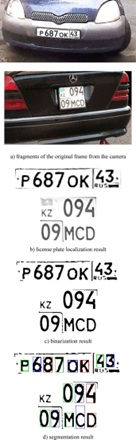
\includegraphics[width=.25\textwidth]{figures/ml.jpg}
    \caption{Resultados del algoritmo de reconocimiento de matrículas\\
    \footnotesize{Fuente: \textit{https://ieeexplore.ieee.org/document/9790745}}}
    \label{fig:ml}
\end{figure}



Los sistemas de reconocimiento de matrículas se pueden adaptar a un amplio rango de características; como Hasan Aljzaere et Al. \cite{10804754}, que desarrollan un sistema de reconocimiento en carreteras utilizando las tecnologías de \textbf{YOLOv8} y \textbf{EasyOCR}. Para probar este sistema, se ha extraído un dataset de 4000 imágenes en blanco y negro de vehículos alemanes de la página web \textbf{Roboflow}. El sistema empieza por detectar los vehículos que aparecen en los vídeos, con el uso del algoritmo SORT \textit{(Simple Online and Real-time Tracking Algorithm)} manteniendo la asociación entre el vehículo y la matrícula. Después de seguir al vehículo, se usará el sistema YOLO para detectar las matrículas, y, si la confianza en la detección supera el 85\%, triplicando su tamaño para pasarlo al algoritmo EasyOCR.

La estructura del extractor de características del modelo YOLOv8 se divide en 3 partes fundamentales: CSB, C2f y SPPF. El módulo \textbf{CSB} con convoluciones 2D y la función de activación SiLU \textbf{ayuda en la extracción de características}, \textbf{C2f mejora el flujo del gradiente} y SPPF se encarga de aprender las características. A esta estructura le sigue el cuello \textbf{PAN-FPN}, \textbf{encargado de} utilizar semántica de alto nivel y la informaciñon de la ubicación para \textbf{mejorar el uso de características}. La última parte es la encargada de separar las tareas de clasificación y detección. 

La tecnología EasyOCR es la encargada de transformar el texto de la imagen en una cadena de caracteres a través de librería de OpenCV, \textbf{comparando la imagen recortada con una plantilla guardada en una base de datos} (similar a la funcionalidad Template Matching), detectando texto en más de 80 lenguajes diferentes, en escenarios donde la orientación de caracteres puede ser compleja. Un ejemplo se puede ver sobre la figura \ref{fig:eocr-ex}.

Este sistema da como resultados una precisión del \textbf{95\%} para la detección de matrículas y un índice de reconocimiento del \textbf{94\%} usando una confianza en el algoritmo EasyOCR del 85\%. El entrenamiento ha consistido de 1000 iteraciones

\begin{figure}[htb]
\centering
    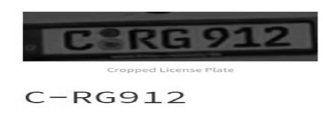
\includegraphics[width=.5\textwidth]{figures/eocr-ex.jpg}
    \caption{Ejemplo de reconocimiento de matrícula usando el algoritmo EasyOcr\\
    \footnotesize{Fuente: \textit{https://ieeexplore.ieee.org/document/10804754}}}
    \label{fig:eocr-ex}
\end{figure}



Para la detección y reconocimiento de matrículas en entornos restringidos y vehículos que rompen las leyes de tráfico, Debajit Sarma et Al.\cite{10710693} idean un sistema de tres partes fundamentales:
\begin{itemize}
    \item \textbf{Detección de la matrícula:} Se convierte la imagen de RGB a binaria (más eficiente computacionalmente), mejorando y suavizando la imagen con el uso de \textit{Gaussian Blurring} para eliminar el ruido; a esto le sigue la aplicación del umbral adaptativo \textit{(Adaptive Thresholding)}.
    \item \textbf{Segmentación de caracteres:} La imagen \ref{fig:plate-seg} detalla los pasos involucrados en esta etapa; fundamental para la siguiente etapa ya que si no se pueden segmentar los caracteres, tampoco se pueden reconocer.
    \item \textbf{Reconocimiento de caracteres:} Un framework de tensorflow junto con una CNN se encargan de reconocer las 36 clases (A-Z y 0-9). La CNN está compuesta de \textbf{3 capas convolucionales} con kernels de 5x5 y \textbf{2 capas totalmente conectadas}; de las cuales, una de ellas con un \textit{dropout} de 0.5 para prevenir el \textit{overfitting}. La red termina con una capa de \textit{softmax} para dar las probabilidades por clase.
\end{itemize}

Para probar el sistema propuesto se han escogido dos conjuntos de datos: el primero\footnote{El conjunto de datos es descargable de la página \href{https://www.kaggle.com/datasets/andrewmvd/car-plate-detection}{CarPlateDetection}} consta de 443 imágenes de vehículos con diferentes condiciones de visibilidad y ángulos con la matrícula visible. El segundo contiene un subconjunto recortado de 1980 imágenes de caracteres y letras\cite{visapp09} (3410 en total) resultando en 55 imágenes por caracter con 45/10 para los conjuntos de entrenamiento y validación. Las pruebas indican un 95.75\% de precisión en el conjunto de caracteres.

\begin{figure}[htb]
\centering
    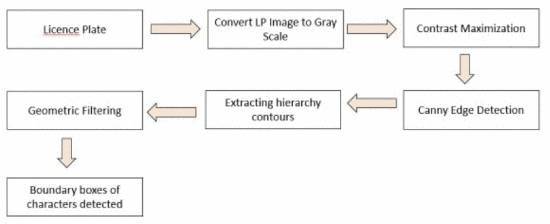
\includegraphics[width=.85\textwidth]{figures/plate-seg.jpg}
    \caption{Proceso de flujo de segmentación de matrículas\\
    \footnotesize{Fuente: \textit{https://ieeexplore.ieee.org/document/10183638}}}
    \label{fig:plate-seg}
\end{figure}



Phayung Meesad et Al.\cite{Meesad2025} combinan el algoritmo \textbf{YOLOv10} con un motor \textbf{Tesseract OCR} especialmente personalizado para la tarea de reconocimiento automatizado de matrículas (ALPR), fundamental para la gestión del tráfico, proteger la seguridad pública, peajes y el acceso a lugares restringidos. La combinación de estos dos algoritmos tiene como objetivo reconocer matrículas de vehículos con una mezcla de \textbf{caracteres tailandeses y latinos}, un problema complicado no resuelto en la literatura. El sistema propuesto toma como entrada imágenes o vídeo en tiempo real de cámaras de vigilancia y se somete a varias \textbf{funciones de preprocesamiento}: reducción del ruido, ajuste del contraste y técnicas de segmentación, que tienen mucha eficacia a la hora de asolar regiones de las matrículas.

La parte de detección utiliza \textbf{modelos YOLO} avanzados ("avanzados" en su momento como YOLOv8, YOLOv9 o YOLOv10) para detectar las matrículas de las imágenes preprocesadas. Después de que la detección resulte correcta, un motor \textbf{Tesseract OCR}, adaptado a matrículas Tailandesas que presentan dos tipos de escritura y fuentes variables para mejorar el reconocimiento y solucionar los problemas lingüísticos inherentes en el conjunto de datos. El modelo \textbf{YOLOv10} destaca entre los modelos comparados en este estudio, característico gracias a sus \textbf{kernels dinámicos convolucionales (DCK)}, que mejora el proceso de extracción de características a costa de un mínimo aumento de la carga computacional. 

El conjunto de datos consta de 50,000 imágenes y 10,000 trozos de vídeo (con una división de 80:20 para los conjuntos de entrenamiento y pruebas) en diferentes condiciones atmosféricas y de iluminación y con cambios notables en las matrículas con colores o fuentes, por ejemplo. Algunos ejemplos se pueden observar en la figura \ref{fig:thai-ex}. Las pruebas realizadas se llevaron a cabo en una NVIDIA A100 GPU de Google Colab comparando los detectores YOLOv5, YOLOv8, YOLOv9, YOLOv10, Faster R-CNN y SSD, cuyos resultados están descritos en la tabla \ref{tab:thai-res} y muestran la superioridad de YOLOv10 frente a los anteriores modelos YOLO. El reconocimiento también tuvo resultados satisfactorios: el motor Tesseract OCR alcanzó una tasa de reconocimiento del 99.16\% y un F1-score del 99.2\%.

\begin{figure}[htb]
\centering
    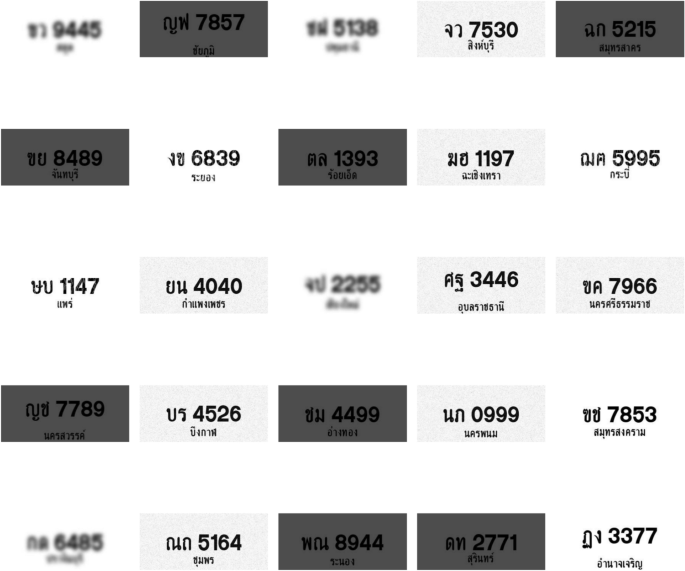
\includegraphics[width=.5\textwidth]{figures/lic-ex.png}
    \caption{Ejemplos de matrículas tailandesas\\
    \footnotesize{Fuente: \textit{https://www.nature.com/articles/s41598-025-24967-9}}}
    \label{fig:thai-ex}
\end{figure}

\begin{table}[htb]
    \centering
    \begin{tabular}{|c|c|c|c|c|c|}
         \hline   
         \textbf{Modelo} & \textbf{Accuracy} & \textbf{Precision} & \textbf{Recall} & \textbf{F1-score} & \textbf{Inference time}\\
         \hline
         \textbf{YOLOv5} & 96.97\% & 97.90\% & 97.10\% & 97.5\% & 1.4 ms\\ 
         \hline
         \textbf{YOLOv8} & 97.79\% & 98.20\% & 97.30\% & 97.7\% & 1.4 ms\\ 
         \hline
         \textbf{YOLOv9} & 98.96\% & 99.8\% & 97.80\% & 98.8\% & 1.4 ms\\ 
         \hline
         \textbf{YOLOv10} & 99.16\% & 99.8\% & 98.60\% & 99.2\% & 1 ms\\ 
         \hline
         \textbf{Faster R-CNN} & 92\% & 92.50\% & 92\% & 92.2\% & 4.5 ms\\ 
         \hline
         \textbf{SSD} & 90\% & 91\% & 90.5\% & 90.7\% & 2.5 ms\\ 
         \hline
    \end{tabular}
    \caption{Resultados de diferentes arquitecturas en el reconocimiento de matrículas tailandesas}
    \label{tab:thai-res}
\end{table}



La gestión del aparcamiento urbano es un problema creciente debido a la limitación del espacio, con los métodos tradicionales fallando en los momentos con mayor tráfico y resultando en ineficiencias, uso inautorizado y pérdidas de dinero. El sistema propuesto por Gulmini Pradhan et Al.\cite{Pradhan2025} considera una cámara con una resolución mínima de 1080 con enfoque automático y HDR visualizando múltiples plazas de aparcamiento (incluyendo visión clara de las matrículas). Cuando el vehículo entra a la plaza, es detectado por un \textbf{sensor IR} que activa la \textbf{cámara}, la cual captura la matrícula. Después de que un modelo \textbf{YOLO} detecte el vehículo y compare su posición con la de la plaza, se verifica la información y se procede a capturar la matrícula y empezar el contador. Después de la verificación, la matrícula se captura usando la tecnología \textbf{OCR} y vinculándola con la base de datos de los vehículos. 

Se aplica \textit{Gaussian Blurring} y \textit{thresholding} (aplicación de un umbral para convertir una imagen en binario) tanto en la imagen del vehículo como en la de la matrícual para reducir el ruido y segmentar la imagen, seguido de un contorneado para localizar y dibujar una bounding box alrededor de una matrícula. Gracias a la aplicación de estas técnicas en la imagen de la matrícula, se puede extraer el texto mejorado con la tecnología Tesseract OCR.

Tesseract OCR es un motor óptico de reconocimiento de texto desarrollado por Google que analiza las características estructurales del texto, resultando en el reconocimiento de patrones en la imagen y transformándola en texto legible para la computadora. Énfasis en los sofisticados algoritmos de reconocimiento que disciernen los caracteres del resto de los elementos visuales irrelevantes en la imagen. Su versatilidad y fiabilidad hacen que sea una herramienta eficaz para una multitud de tareas e industrias que involucran el reconocimiento de texto.

El sistema es eficaz tanto en los entornos con buena visibilidad como con baja, tal y como se puede apreciar en la figura \ref{fig:tocr-ex}, manteniendo una precisión en torno al \textbf{95\%} en condiciones de día y un \textbf{90\%} en condiciones de noche.

\begin{figure}[htb]
\centering
    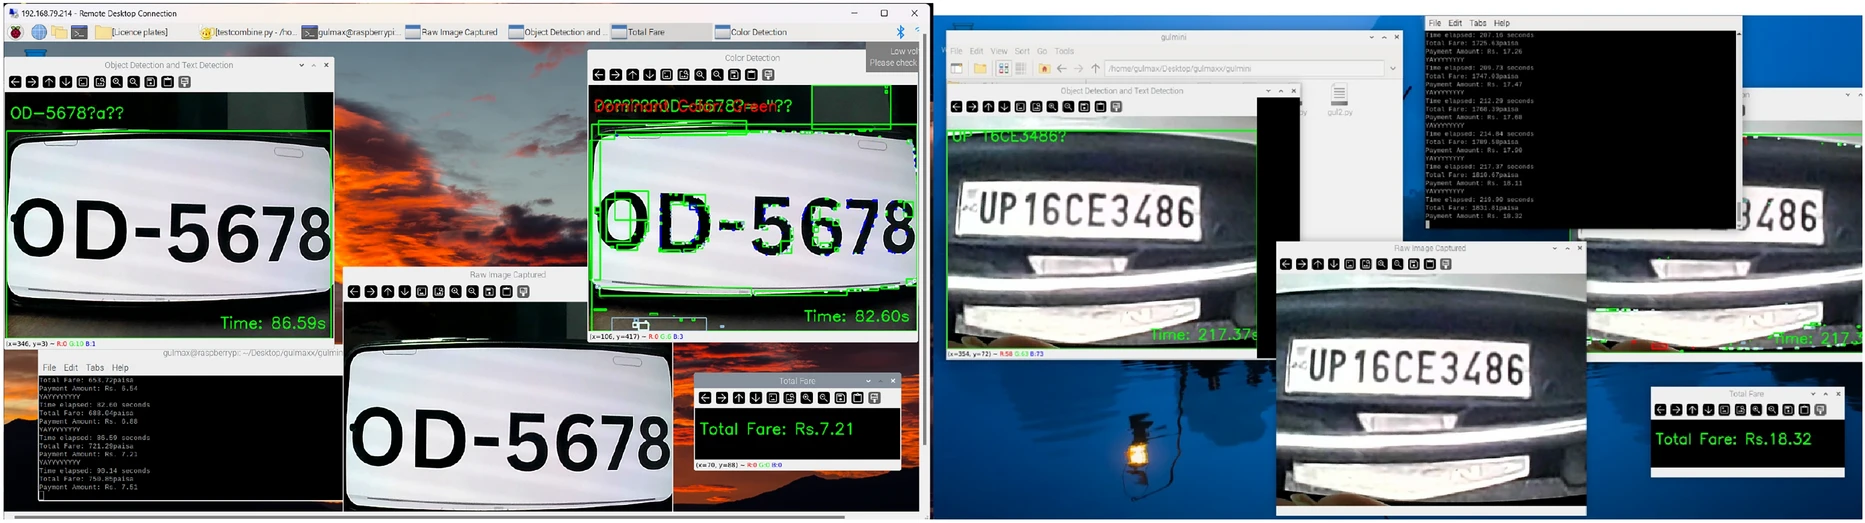
\includegraphics[width=.75\textwidth]{figures/tocr-ex.png}
    \caption{Resultado de Tesseract OCR en varias matrículas\\
    \footnotesize{Fuente: \textit{https://www.nature.com/articles/s41598-025-86441-w}}}
    \label{fig:tocr-ex}
\end{figure}



Hanae Moussaoui et Al.\cite{Moussaoui2024} proponen un nuevo sistema de detección y reconocimiento de matrículas usando el modelo \textbf{YOLOv8}, técnicas de procesamiento de imágenes y una técnica OCR para el reconocimiento de texto; el sistema completo se puede observar sobre la figura \ref{fig:sys-easyocr}.El conjunto de datos se crea a partir de \textbf{270} imágenes de Internet y \textbf{CVAT} (Computer Vision Annotation Tool), un programa de código abierto para etiquetar imágenes y vídeos. Estas imágenes contienen vehículos visibles desde distintos ángulos y varias condiciones de iluminación y se dividen en los subconjuntos de entrenamiento, validación y pruebas.

La matrícula detectada por el modelo \textbf{YOLOv8} se redimensiona y mejora usando técnicas de preprocesamiento, como \textit{k-means clustering}, \textit{thresholding} y operaciones morfológicas. Este paso es crucial para reconocer los caracteres del texto, sobre todo con el ruido producido por la detección de bordes. De entre los modelos YOLO, se escoge la última versión de YOLO (hasta el momento de hacer el artículo), \textbf{YOLOv8}, debido a las mejoras en eficiencia y rendimiento como la introducción de \textbf{NMS (Non-Maximum Suppression)}, que redefine las bounding boxes con baja confianza o duplicadas. Algunos ejemplos de detección sobre varias matrículas se pueden observar en la figura \ref{fig:yolo8-ex}. De entre todas las técnicas \textbf{OCR}, se ha seleccionado \textbf{EasyOCR}, debido a su rápido procesamiento en tiempo real y simple uso en muchos programas en Python.

Los resultados logran alcanzar una precisión del \textbf{74\%} en 40 iteraciones y un 96.37\% al cabo de 68 iteraciones.

\begin{figure}[htb]
\centering
    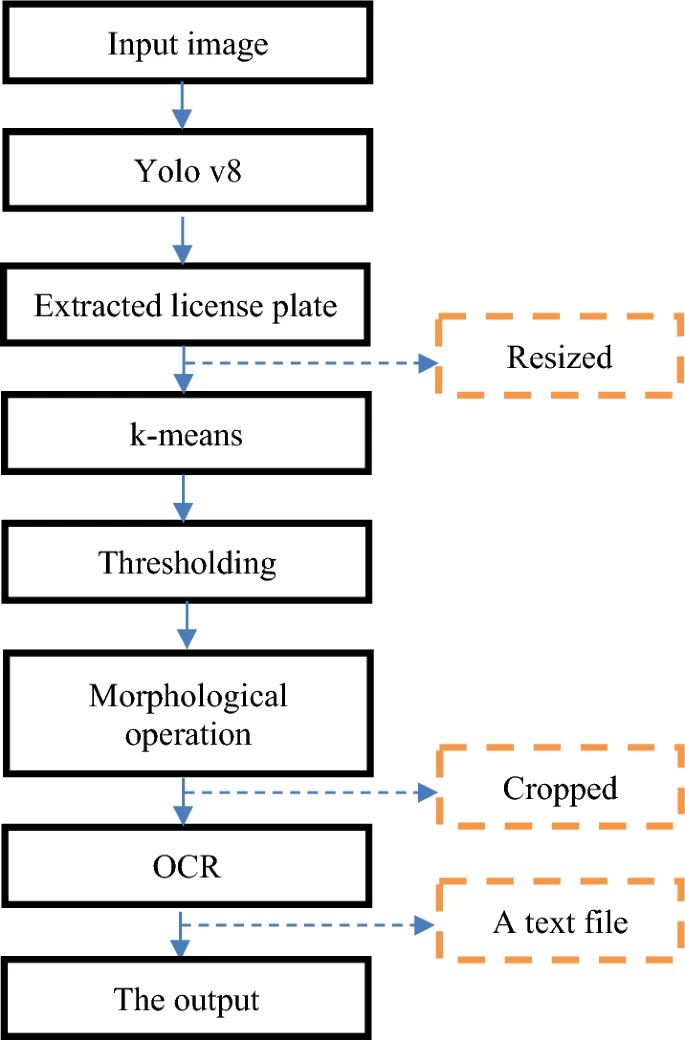
\includegraphics[width=.35\textwidth]{figures/sys-easyocr.png}
    \caption{Flujo del sistema de reconocimiento de matrículas con YOLO, técnicas de preprocesamiento y OCR\\
    \footnotesize{Fuente: \textit{https://www.nature.com/articles/s41598-025-86441-w}}}
    \label{fig:sys-easyocr}
\end{figure}

\begin{figure}[htb]
\centering
    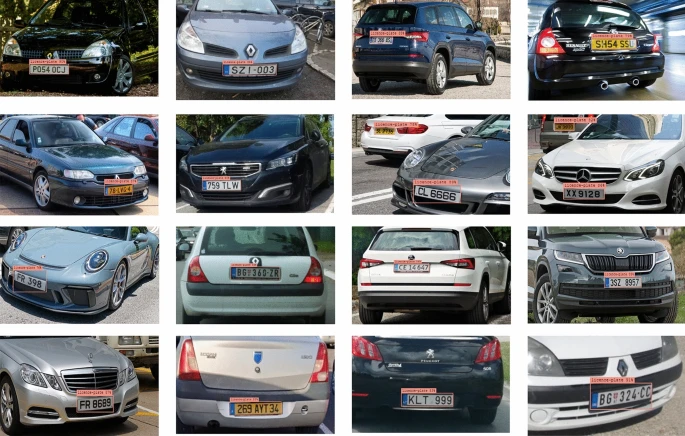
\includegraphics[width=.75\textwidth]{figures/yolo8.png}
    \caption{Ejemplos de detección de matrículas usando el modelo YOLOv8\\
    \footnotesize{Fuente: \textit{https://www.nature.com/articles/s41598-025-86441-w}}}
    \label{fig:yolo8-ex}
\end{figure}



La expansión incesante de las ciudades se ha visto beneficiada por mejoras en cuestiones como la ciencia y la tecnología, lo que resulta en un crecimiento del número de vehículos en los núcleos de población, incluyendo Corea del Sur. Esto da pie al problema descontrolado del acceso a un aparcamiento, incluyendo espacios para gente con discapacidad (plazas para minusválidos). Para abordar este problema, Dhiraj Neupane et Al.\cite{neupane2023shinedeeplearningbasedaccessible} idean \textit{Shine}: un sistema de detección novedoso del vehículo, la matrícula (incluido el reconocimiento de los caracteres), y las pegatinas o marcas de vehículos para deshabilitados. La metodología completa que se ha llevado a cabo en este trabajo se puede dividir en:
\begin{itemize}
    \item \textbf{Recolección de datos:} 30,000 imágenes de vehículos coreanos y de placas de acceso fueron recogidas de plazas de aparcamiento, páginas del gobierno y conjuntos de datos online. Estas marcas se pueden encontrar en cualquier ángulo por lo que se ha aplicado \textit{Data Augmentation} con rotaciones de hasta 60 grados con intervalos de 30. 
    \item \textbf{Etiquetado:} Unas 29,000 imágenes se anotaron con el formato YOLO y el formato Pascal VOC para detección de objetos con la herramienta \textbf{makesense.ai}. Las imágenes ya anotadas se dividieron en conjuntos de entrenamiento y validación con una proporción de 90/10. El número de clases en el conjunto es de 69 incluyendo el vehículo, el tipo de matrícula (4 tipos), caracteres alfanuméricos y las marcas, como se puede observar en la figura \ref{fig:cl-dist}.
    \item \textbf{Entrenamiento y pruebas:}  Especificamente se entrenaron los modelos YOLOv4, YOLOv5s, YOLOv7 y Faster R-CNN a través de \textit{Transfer Learning}, permitiendo usar los modelos preentrenados para adaptarse a esta tarea (o a cualquier otra). Los resultados dispuestos en la tabla \ref{tab:res-shame} demuestran la superioridad de YOLOv7 en cuestión de precision de detección frente a modelos más antiguos YOLO y a Faster R-CNN; sin embargo YOLOv5 supera a todos los demás en cuestión de inferencia por imagen. Finalmente, se termina eligiendo el modelo YOLOv7 debido a la prioridad por la precisión y una velocidad de inferencia aceptable para el proyecto. 
    \item \textbf{Post-procesado:} Después de aplicar la deteción con YOLOv7, el resultado es procesado por medio de matemática simple para sacar la matrícula y los números de las marcas, mostrado en la figura \ref{fig:shine-example}.
\end{itemize}

La figura \ref{fig:shine} provee toda la información acerca del funcionamiento del sistema Shine, incluyendo los componentes, el trabajo y los algoritmos, donde (a) enseña los contenidos el hardware completo del sistema, (b) la operación a seguir a partir de una imagen y (c) una demostración del post-procesado que se lleva a cabo para verificar los derechos de accesibilidad del vehículo.

\begin{figure}[htb]
\centering
    \includegraphics[width=.85\textwidth]{figures/cl-dist.png}
    \caption{Distribución de clases del conjunto de datos del sistema Shine\\
    \footnotesize{Fuente: \textit{https://arxiv.org/pdf/2302.00837}}}
    \label{fig:cl-dist}
\end{figure}

\begin{table}[htb]
    \centering
    \begin{tabular}{|c|c|c|c|c|c|}
         \hline   
         \textbf{Modelo} & \textbf{mAP50} & \textbf{mAP50-95} & \textbf{Precision} & \textbf{Recall} & \textbf{Inference time}\\
         \hline
         \textbf{YOLOv7} & 92.16\% & 66.57\% & 94.7\% & 90.84\% & 60ms\\ 
         \hline
         \textbf{YOLOv5s} & 87.77\% & 62.13\% & 94.51\% & 83.08\% & 12.63ms\\ 
         \hline
         \textbf{YOLOv4} & 83.17\% & \- & 92\% & 87\% & 260.1ms\\ 
         \hline
         \textbf{Faster R-CNN} & 70.50\% & \- & 69.94\% & 72.9\% & 292.33ms\\ 
         \hline
    \end{tabular}
    \caption{Resultados de los modelos de detección usados en el sistema Shine}
    \label{tab:res-shame}
\end{table}

\begin{figure}[htb]
\centering
    \includegraphics[width=.75\textwidth]{figures/shine-example.png}
    \caption{Post-procesado de (a) Matrícula (b) Marca\\
    \footnotesize{Fuente: \textit{https://arxiv.org/pdf/2302.00837}}}
    \label{fig:shine-example}
\end{figure}

\begin{figure}[htb]
\centering
    \includegraphics[width=.85\textwidth]{figures/shine.png}
    \caption{Componentes del sistema Shine\\
    \footnotesize{Fuente: \textit{https://arxiv.org/pdf/2302.00837}}}
    \label{fig:shine}
\end{figure}



La identificación automática de matrículas de vehículos se pueden usar para comparar dichas matrículas con bases de datos de vehículos robados, sin seguro, criminales,... La tecnología de OCR \textit{(Optical Character Recognition)} es una de las más explotadas para reconocer matrículas y aunque, es muy eficaz, tiene varias limitaciones como el ruido, las condiciones atmosféricas, la luz o la oclusión ambiental. Para reparar este hueco, Nouar AlDahoul et Al.\cite{aldahoul2024advancingvehicleplaterecognition} proponen el uso de modelos de lenguaje visual (VLMs) como \textit{OpenAI GPT4o}, \textit{Google Gemini 1.5} o \textit{Anthropic Claude 3.5 Sonnet} en un trabajo comparativo junto con un VLM propio: VehiclePaliGemma. Los conjuntos de datos que se van a utilizar son:
\begin{itemize}
    \item \textbf{Complex Plate Dateset:} 258 imágenes de matrículas malayas que están borrosas, difíciles de reconocer para los métodos de OCR y que sólo se utilizarán para evaluar el modelo.
    \item \textbf{Training Plate Dateset:} 600 imágenes sintéticas para hacer fine-tuning al modelo \textit{PaliGemma}, cada una con un tamaño de 120 x 50 píxeles, rotadas en 5 grados, se difuminaron y se sometieron a ruidos Gaussianos y "sal y pimienta".
    \item \textbf{Diverse Car Dateset:} 140 imágenes extraídas de Internet etiquetadas por mayoría en votación 3 modelos distintos 
\end{itemize}
La solución propuesta es una combinación de Inteligencia Artificial de procesado lenguaje y visual de las VLMs para entender los caracteres sin necesidad de preprocesado. El diagrama de la solución se puede observar en la figura \ref{fig:vlms}. Después de incluir en las pruebas de reconocimiento 3 modelos de OCR: EasyOCR, KerasOCR y Tesseract, los resultados observados en la figura \ref{tab:res-vlms} indican que estos modelos OCR que mostraban buenos resultados en este tipo de tareas, fallan al intentar reconocer las imágenes del dataset \textbf{Malaysian license plates}\footnote{Tesseract está basado en redes LSTM, EasyOCR usa el algoritmo Character-Region Awareness for Text detection (CRAFT) junto con RCNNs y KerasOCR usa el algoritmo CRAFT usa RCNNs o transformadores.}. De entre los VLMs preentrenados, GPT-4o destaca reconociendo correctamente 222 de las 258 matrículas, seguido de su versión más pequeña, GPT-4o, y superando ambos con una buena diferencia al resto de VLMs, sean pequeñas o grandes. 

Sin embargo, el modelo que destaca es VehiclePaliGemma, identificando 226 matrículas correctamente; una diferencia considerable con su modelo sin hacer \textit{fine-tuning}, que sólo pudo identificar 178. Además el modelo es capaz de predecir la matrícula de un vehículo a una velocidad de 7 FPS en una A100-80GB GPU. Para analizar más en profundidad los resultados es necesario observar la figura \ref{fig:vlms-cm}, donde los modelos fallan más al intentar identificar los caracteres. 

Cuanto más claro sea una celda, menos veces ha conseguido el modelo identificar ese caracter correctamente. De aquí se pueden sacar observaciones como que la "I" tiene muchos problemas para ser identificada por algunos modelos, pero por otros es totalmente lo contrario o, la más evidente, que todos los modelos tienen problemas para identificar el caracter "Q".

\begin{figure}[htb]
\centering
    \includegraphics[width=.75\textwidth]{figures/vlms.png}
    \caption{Diagrama de uso de VLMs para reconocer caracteres en matrículas\\
    \footnotesize{Fuente: \textit{https://arxiv.org/pdf/2412.14197}}}
    \label{fig:vlms}
\end{figure}

\begin{table}[htb]
    \centering
    \begin{tabular}{|c|c|c|}
         \hline   
         \textbf{Modelo} & \textbf{Matrículas correctamente predichos} & \textbf{Precisión (\%)}\\
         \hline
         \textbf{EasyOCR} & 79 & 32.95\%\\ 
         \hline
         \textbf{Tesseract} & 97 & 36.74\%\\ 
         \hline
         \textbf{KerasOCR} & 107 & 40.53\%\\ 
         \hline
         \textbf{moondream2} & 102 & 39.5\%\\ 
         \hline
         \textbf{VILA} & 144 & 55.8\%\\ 
         \hline
         \textbf{LLaVA-NeXT-7b} & 147 & 57\%\\ 
         \hline
         \textbf{Gemini 1.5 flash} & 200 & 77.5\%\\ 
         \hline
         \textbf{GPT-4o-mini} & 220 & 85.7\%\\ 
         \hline
         \textbf{LLaVA-NeXT-34b} & 152 & 58.9\%\\ 
         \hline
         \textbf{Gemini 1.5 Pro} & 185 & 71.7\%\\ 
         \hline
         \textbf{GPT-4o} & 222 & 86\%\\ 
         \hline
         \textbf{Llama 3.2 Instruct} & 175 & 67.83\%\\ 
         \hline
         \textbf{Claude 3.5 Sonnet} & 186 & 72.1\%\\ 
         \hline
         \textbf{Pre-trained PaliGemma} & 178 & 69\%\\ 
         \hline
         \textbf{VehiclePaliGemma} & 226 & 87.6\%\\ 
         \hline
    \end{tabular}
    \caption{Resultados de diferentes VLMs en reconocimiento de matrículas}
    \label{tab:res-vlms}
\end{table}

\begin{figure}[htb]
\centering
    \includegraphics[width=.85\textwidth]{figures/vlms-cm.png}
    \caption{Mapa de calor de la precisión de reconocimiento de caracteres en diferentes VLMs.\\
    \footnotesize{Fuente: \textit{https://arxiv.org/pdf/2412.14197}}}
    \label{fig:vlms-cm}
\end{figure}



Con la idea de gestionar de manera eficiente el tráfico, la seguridad, el reconocimiento de vehículos y los aparcamientos, Sergey Zherzdev y Alexey Gruzdev\cite{zherzdev2018lprnetlicenseplaterecognition} crean el primer método en tiempo real de reconocimiento de matrículas que no use RNNs, \textbf{LPRNet}. Estudios previos sugerían el uso de los modelos VGG, ResNet o GoogLeNet para esta tarea; en vez de eso, se construye una red neuronal inspirada en los "bloques de fuego" de SqueezeNet y los bloques de Inception. El diseño consta de varias partes:
\begin{itemize}
    \item Preprocesamiento con una red de ubicación (LocNet), visible en la figura \ref{fig:locnet}, con una \textbf{capa de transformación espacial}  para conseguir mejores características.
    \item El extractor de características de la figura \ref{fig:lprnet-backbone} (donde el bloque básico es el de la figura \ref{fig:lprnet-basicblock}) permite \textbf{extraer las características espacialmente distribuidas}. El kernel de la última capa convolucional (1x13) utiliza el contexto local en vez del LSTM de las RNNs.
    \item Clasificación de los caracteres por cada posición.
    \item Procedimiento post-filtro, que devuelve las N secuencias más probables encontradas por \textit{Beam Search} y devuelve la que más encaje con unas marcas predefinidas según las regulaciones locales para las matrículas.
\end{itemize}

\begin{figure}[htb]
\centering
    \includegraphics[width=.5\textwidth]{figures/locnet.png}
    \caption{Red de ubicación (LocNet)\\
    \footnotesize{Fuente: \textit{https://arxiv.org/pdf/1806.10447}}}
    \label{fig:locnet}
\end{figure}

\begin{figure}[htb]
\centering
    \includegraphics[width=.5\textwidth]{figures/lprnet-backbone.png}
    \caption{Extractor de características del modelo LPRNet\\
    \footnotesize{Fuente: \textit{https://arxiv.org/pdf/1806.10447}}}
    \label{fig:lprnet-backbone}
\end{figure}

\begin{figure}[htb]
\centering
    \includegraphics[width=.5\textwidth]{figures/lprnet-basicblock.png}
    \caption{Bloque básico del extractor de características del modelo LPRNet\\
    \footnotesize{Fuente: \textit{https://arxiv.org/pdf/1806.10447}}}
    \label{fig:lprnet-basicblock}
\end{figure}

El entrenamiento se ha realizado con la herramienta de Tensorflow, usando el optimizador Adam, una tasa de aprendizaje de 0.001 y una escala de ruido del gradiente de 0.001. La tasa de aprendizaje se reduce en un 10\% cada 100,000 iteraciones, entrenándose el modelo con 250,000 iteraciones en total. La red de ubicación LocNet se activa a partir de la iteración 5,000, ya que al principio del entrenamiento puede llevar a degradar los resultados al no poder recibir correctamente los gradientes. El dataset seleccionado fue el Chinese License Plates dataset, con 11696 imágenes de matrículas, donde el modelo pudo alcanzar un \textbf{95\%} tardando 3 ms por cada imagen con el uso de una NVIDIA GTX 1080 o 1.3 ms usando una CPU Intel Core i7-6700K.



En cualquier tarea de detección de objetos, el uso de múltiples puntos de vista puede ayudar a resolver muchos problemas de baja visibilidad. Dat Tran-Anh et Al.\cite{trananh2023licenseplaterecognitionbased} idean un método de detección de texto en las matrículas utilizando 3 puntos de vista diferentes para restaurar los componentes de la matrícula basándose en estimaciones de nivel y distancias. El flujo del reconocimiento de matrículas tiene dos partes indivisibles: la detección de objetos dentro de la imagen (en este caso particular, la propia matrícula, algún elemento substancial del vehículo o, el propio vehículo) y el reconocimiento de los caracteres en la matrícula. Este trabajo consta de 3 partes:
\begin{itemize}
    \item Detección del vehículo y la matrícula con el modelo YOLOv8, elegido gracias a su alta precisión y velocidad de inferencia. Se recolectaron imágenes de vehículos con las matrículas visibles para crear un dataset propio. Si se detecta la matrícula, el trozo de imagen con esta \textbf{se recorta y se envía a la parte 2}.
    \item Se crea una una \textbf{nueva función de coste basada en la métrica IoU para solventar predicciones de matrícula de menor tamaño que el real}. Dadas dos imágenes I1 e I2, un modelo DenseNet se entrena para producir una imagen fusionada con la mayor calidad posible. Se computan dos valores w1 y w2 como el grado de preservación de la información, a partir de aplicar la función softmax a la división entre la información y el número de clases. La función de pérdida final queda definida como $L = E(w_1 * MSE_{If, I1} + W_2 * MSE_{If, I2})$, que se usará para entrenar el modelo de agregación de características: el cual combina características de varios fotogramas en una única representación para el reconocimiento de matrículas.
    \item La arquitectura \textbf{CnOCR}, cuya arquitectura se puede observar en la figura \ref{fig:ocr-arc}, tiene una inferencia por imagen de solo 0.03 segundos. Se empieza con \textbf{múltiples capas convolucionales y capas de agregación} a los que le sigue una capa de \textbf{LSTM bidireccional de 100 nodos} que se encarga de capturar la información contextual y las dependencias entre caracteres. La última capa es una densa con activación \textit{softmax} de 53 caracteres.
\end{itemize}
El conjunto de datos creado es \textbf{PTITPlates}, que fue etiquetado con la herramienta LabelMe, con imágenes de carreteras y zonas industriales con diferentes puntos de vista. El método propuesto logra alcanzar un \textbf{91.3\%} de f1-score en el dataset PTITPlates y un \textbf{90.8} de f1-score en el dataset de Stanford Cars.

\begin{figure}[htb]
\centering
    \includegraphics[width=.75\textwidth]{figures/ocr-arc.png}
    \caption{Arquitectura OCR\\
    \footnotesize{Fuente: \textit{https://arxiv.org/pdf/2309.12972}}}
    \label{fig:ocr-arc}
\end{figure}



Los sistemas de identificación de matrículas requieren ser resielientes a cambios, debido al cambio constante y la cantidad constante de nuevas matrículas registradas al tráfico. Los métodos que usan transformadores exceden en este trabajo sin ningún problema, hasta recientemente, que su rendimiento no para de reducirse considerablemente. Florent Meyer et Al.\cite{Meyer_2025} idean un transformador, \textbf{SaLT} que pueda identificar futuras matrículas con diferentes secuencias con el uso de varias modificaciones. El modelo base seleccionado es TrOCR\footnote{El modelo es accesible por: \url{https://huggingface.co/docs/transformers/model_doc/trocr}}, el cual tiende a aprender la estructura exacta de las matrículas del conjunto de entrenamiento. 

La primera propuesta es \textbf{cambiar el codificador del transformador por una FCN (Fully Convolutional Network)} para descartar la información posicional (intrínsecamente ligada al transformador); en vez de eso, esta FCN extrae las características de las imágenes sin este problema. Aquí surge otro problema: las redes convolucionales tienen problemas para capturar relaciones entre píxeles a largo plazo, especialmente al usar kernels de pequeño tamaño, como ResNet, así que \textbf{se reduce su uso hacia pequeños bloques que sólo se encarguen de retener la información y representación de un sólo caracter}, de modo que los rasgos de un caracter determinado no dependa de sus adyacentes. 

La segunda modificación es en el decodificador, cuya parte no es eliminada (es necesaria para el reconocimiento de los caracteres), sino que se empieza por \textbf{eliminar los "token embeddings" del texto de la entrada y sustituirlos por una secuencia de colas posicionales que contienen solamente codificaciones posicionales}. Lo siguiente es \textbf{eliminar estas últimas conexiones en la última capa}, de forma que no se dé el problema del desvanecimiento del gradiente y que además previene que justo antes de la capa de predicción se elimine la información de la posición. Gracias a eliminar la dependencia de la posición al finalizar, la última capa devuelve unas características sin posición.

Los conjuntos de datos propuestos son: un nuevo dataset sintético LPR-MNIST y el dataset LP. \textbf{LPR-MNIST} es una colección de 100,000 pares de imagen/texto concatenando 5 dígitos en blanco sobre fondo negro del dataset MNIST (cuyas imágenes fueron redimensionadas a 32 x 32 píxeles y seleccionadas aleatoriamente para cada dato del dataset, como se puede observar en la figura \ref{fig:lpr-mnist}), siendo los números del dataset desde 00000 hasta 99999. El dataset \textbf{LP} contiene 797,469 y 97,725 para los conjuntos de entrenamiento y validación, respectivamente. Este nuevo transformador modificado logra alcanzar un \textbf{97.3\%} de precisión en el dataset LP, contrastando de manera significativa con los 27.8\% del transformador TrOCR.

\begin{figure}[htb]
\centering
    \includegraphics[width=.75\textwidth]{figures/lprmnist.png}
    \caption{Ejemplos del dataset LPR-MNIST\\
    \footnotesize{Fuente: \textit{https://arxiv.org/pdf/2506.17051}}}
    \label{fig:lpr-mnist}
\end{figure}



El coste computacional de las CNNs limitan su uso en sistemas de reconocimiento de matrículas. El trabajo presentado por George B. Nardes et Al.\cite{NARDES2026102654}, presenta una CNN de 8 bits cuantificados diseñada para el reconocimiento óptico de caracteres (OCR) de matrículas de Mercosur y Brasil. Los datasets empleados son SATTRA y UFPR-ALPR\footnote{El dataset es accesible por: \url{https://github.com/raysonlaroca/ufpr-alpr-dataset}}, que juntos acaban siendo 82308/3500/13300 imágenes para cada conjunto, respectivamente, y una distribución de clases no balanceada (excepto en el conjunto de validación). 

La arquitectura base seleccionada es LeNet-5, debido a su compactación y bajo número de parámetros, para poder terminar siendo un modelo muy eficiente y portátil cuya arquitectura se puede observar en la figura \ref{fig:lenet}. Las modificaciones aplicadas fueron:
\begin{itemize}
    \item La entrada fue modificada para aceptar \textbf{3 canales de 32 x 24 píxeles}.
    \item Las capas convolucionales se rediseñaron todas para que usen \textbf{kernels de 3 x 3}.
    \item Las 3 últimas capas totalmente conectadas se convierten en una única, reemplazando las dos primeras por una \textbf{capa convolucional y una capa de agrupación} (pooling). La última parte de la arquitectura termina siendo una cabeza FC de 128 x 35, siendo 35 el número de caracteres del conjunto de entrenamiento.
\end{itemize}

\begin{figure}[htb]
\centering
    \includegraphics[width=.85\textwidth]{figures/lenet.jpg}
    \caption{Arquitectura de LeNet-5 modificada\\
    \footnotesize{Fuente: \textit{https://www.sciencedirect.com/science/article/pii/S016792602600009X}}}
    \label{fig:lenet}
\end{figure}

Este modelo logra altos resultados de rendimiento en los datasets de UFPR, con una precisión de \textbf{90.22\%} y una matriz de confusión de la figura \ref{fig:lenet-cm}, y sobre todo en el dataset SATTRA, con una precisión de \textbf{97.11\%}. Comparando rendimiento, aunque se comparan varias GPUs, es notable la comparativa entre los \textbf{1.99ms} y \textbf{502 FPS} de la NVIDIA Titan XP con los \textbf{10.20ms} y \textbf{98 FPS} de la Tesla P100.

\begin{figure}[htb]
\centering
    \includegraphics[width=.85\textwidth]{figures/lenet_cm.jpg}
    \caption{Arquitectura de LeNet-5 modificada\\
    \footnotesize{Fuente: \textit{https://www.sciencedirect.com/science/article/pii/S016792602600009X}}}
    \label{fig:lenet-cm}
\end{figure}




\chapter{Métodos seleccionados}
\label{Métodos seleccionados}

Para este proyecto se han escogido dos implementaciones completamente diferentes para hacer comparaciones entre ellas tanto en el rendimiento como en la precisión en la tarea de detección. Los métodos seleccionados son:

\subsection{YOLOv26n}

YOLO26\cite{sapkota2026yolo26keyarchitecturalenhancements}, publicado en Septiembre de 2025, es la versión más novedosa entre los modelos YOLO, con más mejoras en cuestión de eficiencia, precisión y despliegue en dispositivos de menor rendimiento; algo que se puede observar en la figura \ref{fig:yolo-stats} en comparación con anteriores modelos. 

\begin{figure}[htb]
\centering
    \includegraphics[width=.85\textwidth]{figures/yolo_stats.png}
    \caption{Compensación entre velocidad y precisión entre los distintos modelos YOLO\\
    \footnotesize{Fuente: \textit{https://arxiv.org/pdf/2509.25164}}}
    \label{fig:yolo-stats}
\end{figure}



\subsubsection{Arquitectura de YOLO26}

Esta nueva arquitectura, visible en la figura \ref{fig:yolo26-arch}, elimina el \textit{Distribution Focal Loss} (DFL) \footnote{Función de pérdida que cuantifica el objetivo de la regresión en múltiples celdas o contenedores, permitiendo que sea más flexible la representación de las \textit{bounding boxes}.} e integrando\cite{chakrabarty2026yolo26analysisnmsfreeend}:

\begin{figure}[htb]
\centering
    \includegraphics[width=.85\textwidth]{figures/yolo26_arch.png}
    \caption{Arquitectura del modelo YOLO26 para detección y segmentación\\
    \footnotesize{Fuente: \textit{https://arxiv.org/pdf/2509.25164}}}
    \label{fig:yolo26-arch}
\end{figure}

\begin{itemize}
    \item \textbf{NMS-Free inference End to End:} NMS es una función que elimina \textit{bounding boxes} superpuestas a otras, seleccionando la propuesta con mayor confianza. YOLO26 rediseña la predicción, haciendo que el modelo prediga \textbf{una sola bounding box por cada instancia} durante el entrenamiento. Eliminar esta parte \textbf{mejora en un 43\% la latencia} en el entrenamiento con el uso de la CPU, en donde se hacía un cuello de botella debido a multitud de operaciones secuenciales.
    
    \item \textbf{ProgLoss:} Es una estrategia de pérdida de pesos dinámica. En otros detectores, tiene que haber un balance entre el arreglo por la función de pérdida de clasificación ($L_{cls}$) y el arreglo por la función de pérdida de regresión de la \textit{bounding box} ($L_{box}$), lo que provoca que la red neuronal tenga que aprender a la vez a diferenciar entre características y a localizar con precisión sin el uso de anclajes. 
    
    Este nuevo sistema introduce un coeficiente $\lambda_t$ en la ecuación: 
    \begin{equation*}
        L_{total}(t) = \lambda_t * L{cls} + (1 - \lambda_t) * L_{box}
    \end{equation*}
    lo que resulta en que el aprendizaje prioriza las \textbf{características de alto nivel al principio} del entrenamiento y, \textbf{según progresa el aprendizaje}, este va priorizando \textbf{características geométricas de grano fino}, lo que se puede observar en la figura \ref{fig:progloss}.

    \begin{figure}[htb]
    \centering
        \includegraphics[width=.85\textwidth]{figures/progloss.png}
        \caption{Estrategia de priorización del sistema Progloss\\
        \footnotesize{Fuente: \textit{https://arxiv.org/html/2601.12882v1}}}
        \label{fig:progloss}
    \end{figure}


    \item \textbf{Small-Target-Aware Label Assignment:} STAL es una implementación que nace para solucionar el problema "desvanecimiento del objeto pequeño", donde la dependencia del umbral de IoU de estrategias típicas no funciona en objetos pequeños (ocupando menos de un 1\% de la imagen) debido a la sensibilidad del IoU a pequeñas traslaciones espaciales. STAL, como se define en la siguiente ecuación:     
    
    \begin{equation*}
        \tau_{dynamic} = \tau_{base} * (1 - \alpha * \varepsilon^{-\frac{Area_{obj}}{Area_{img}}})
    \end{equation*}
    
    reemplaza el umbral fijo, que suele ser en torno a 0.5, por un umbral $\tau$ que se reduce según el tamaño del objeto y un parámetro $\alpha$ para la tasa de decaimiento en la que el umbral se reduce.

    \item \textbf{Optimizador MuSGD:} Debido a la eliminación del módulo DFL, es necesario introducir un entrenamiento más robusto que no permita que el descenso del gradiente colapse. Ultralytics introduce a YOLO26 el optimizador MuSGD, un optimizador híbrido que fusiona las propiedades del SGD estándar con el optimizador Muon. Este último realiza una ortogonalización matricial, actualizando la matriz de pesos para que sea ortogonal a su estado actual.

    Definimos el \textit{buffer} del momento estándar $v_t$ usado en SGD
    
    \begin{equation*}
        v_{t+1} = \beta * v_t + g_t
    \end{equation*}
    
    donde $g_t$ es el gradiente y $\beta$ es el coeficiente del momento. MuSGD modifica la última actualización de los pesos usando la \textbf{ortogonalización de Newton-Schulz} \footnote{En lugar de expandir polinomios largos y repetir multiplicaciones sobre dimensiones extensas, se agrupa el proceso iterativo en una estructura unificada que evalúa la contribución real de cada potencia matricial. Al identificar y eliminar términos de escasa relevancia y al permitir que algunos coeficientes sean aprendidos por optimización, se consigue una combinación más parsimoniosa que converge de forma más estable y con menos operaciones pesadas\cite{q2bstudioUNSOOrtogonalizacixF3n}.}, la cual "blanquea" la matriz de gradientes usando un proceso iterativo de refinamiento: 
    \begin{equation*}
        \theta_{t+1} = \theta_t - \eta * (\alpha * v_{t+1} + (1 - \alpha) * NewtonSchulz(g_t))
    \end{equation*}
    Este método \textbf{mitiga la varianza} de SGD mientras \textbf{elimina la inestabilidad de las actualizaciones ortogonales} de Muon: figura \ref{fig:musgd}.

    \begin{figure}[htb]
    \centering
        \includegraphics[width=.85\textwidth]{figures/musgd.png}
        \caption{Concepto visual esperado de la optimización dinámica de MuSGD\\
        \footnotesize{Fuente: \textit{https://arxiv.org/html/2601.12882v1}}}
        \label{fig:musgd}
    \end{figure}
\end{itemize}



\subsubsection{Modelos YOLO}

Aunque YOLO se creó con la principal finalidad de la tarea de detección, se han ido creando distintos modelos a lo largo de las versiones de YOLO con diferentes fines: clasificación, segmentación de instancias, detección de puntos claves/poses y detección de objetos orientados. Actualmente, Ultralytics construye 5 modelos distintos con la misma estructura, aunque con diferentes tamaños de capas. Para esta última versión de detección de YOLO, YOLO26, hay 5 modelos más o menos potentes (dependiendo del número de parámetros), cuyas especificaciones se pueden observar en la tabla \ref{tab:yolo-models} usando imágenes de 640 x 640 píxeles, redimensionadas del conjunto de datos COCO.

\begin{table}[htb]
    \centering
    \begin{tabular}{c|c|c|c|c}
        \hline
        \textbf{Modelo} & \textbf{mAP}$\_{val}$\textbf{50-95} & \textbf{Velocidad T4 TRT10(ms)} & \textbf{Parámetros(M)} & \textbf{FLOPs(B)}\\
        \hline
        \textbf{YOLO26n} & 40.9\% & 1.7 ms & 2.4 M & 5.4 B\\
        \hline
        \textbf{YOLO26s} & 48.6\% & 2.5 ms & 9.5 M & 20.7 B\\
        \hline
        \textbf{YOLO26m} & 53.1\% & 4.7 ms & 20.4 M & 68.2 B\\
        \hline
        \textbf{YOLO26l} & 55.0\% & 6.2 ms & 24.8 M & 86.4 B\\
        \hline
        \textbf{YOLO26x} & 57.5\% & 11.8 ms & 55.7 M & 193.9 B\\
        \hline
    \end{tabular}
    \caption{Resultados de los distintos modelos YOLO26 de detección}
    \label{tab:yolo-models}
\end{table}



\subsection{RT-DETR}

\textbf{RT-DETR}\cite{zhao2024detrsbeatyolosrealtime} es, como su propio nombre indica, el primer detector end-to-end en tiempo real: debido al impacto negativo del uso de la función NMS en los modelos YOLO (anteriores a YOLO26, el cual elimina esta función), estos modelos perdían precisión y velocidad. Estos detectores de objetos se caracterizan por un proceso optimizado cuya base de este algoritmo (DETR)\cite{carion2020endtoendobjectdetectiontransformers} es un detector basado en un transformador que modela la detección de objetos como una tarea de predicción y asigna las etiquetas por emparejamiento de grafos bipartitos\footnote{Forma de emparejar vértices de dos conjuntos diferentes de forma que cada vértice esté conectado por un borde a 1 solo vértice del otro conjunto.}. A pesar de tener bastantes ventajas, DETR sufría de una cconvergencia en el entrenamiento muy lenta, un coste computacional alto y unas colas difíciles de optimizar; algo que los modelos DETR posteriores tratan de solucionar: 
\begin{itemize}
    \item \textbf{Acelerar la convergencia}: Deformable DETR\cite{zhu2021deformabledetrdeformabletransformers} mejora la eficiencia del mecanismo de atención con características multiescala. DAB-DETR\cite{liu2022dabdetrdynamicanchorboxes} y DN-DETR\cite{li2022dndetracceleratedetrtraining} introducen un esquema iterativo de refinamiento y un entrenamiento con supresión de ruido, mientras que Group-DETR\cite{chen2023groupdetrfastdetr} introduce una asignación \textit{one-to-many} por grupos.
    \item \textbf{Reducción del coste computacional}: Efficient DETR\cite{yao2021efficientdetrimprovingendtoend} y Sparse DETR\cite{roh2022sparsedetrefficientendtoend} reducen el número de capas del codificador-decodificador o el número de colas, mientras que Lite DETR\cite{li2023litedetrinterleaved} reduce la frecuencia de actualización de características de bajo nivel de forma intercalada.
    \item \textbf{Optimización de inicialización de las colas}: Conditional DETR\cite{meng2023conditionaldetrfasttraining} y Anchor DETR\cite{wang2022anchordetrquerydesign} reducen la dificultad computacional de las colas, Deformable DETR\cite{zhu2021deformabledetrdeformabletransformers} propone un DETR de doble etapa con un selector de colas mixtas y DINO\cite{zhang2022dinodetrimproveddenoising} aprovecha este mismo selector para inicializar de manera más eficaz las colas.
\end{itemize}

Este modelo, cuya arquitectura se puede observar en la figura \ref{fig:rt-detr}, consiste en un extractor de características (backbone), un codificador híbrido eficiente y un decodificador de transformador con cabezas de predicción auxiliares:
\begin{itemize}
    \item \textbf{Backbone}: Sirve como el extractor de características principal para transformar los píxeles de la imagen en mapas de características multiescala que el codificador puede refinar. Las arquitecturas que se han seleccionado para probarse junto al codificador-decodificador son ResNet50 y ResNet101\cite{he2015deepresiduallearningimage} como sustitutos de los modelos L y X de YOLO; para los modelos más ligeros, como los S y L de YOLO se modifican tanto el backbone (por ResNet34 y ResNet18) y además se modifican el número de capas en el codificador-decodificador.
    
    \item \textbf{Efficient Hybrid Encoder}: El mecanismo de atención de Deformable DETR reduce el coste computacional, pero incrementa la longitud de la secuencia de características multiescala lo que deriva en que el codificador se convierta en un cuello de botella, usando el 49\% de los GFLOPs del modelo y contribuyendo solamente un 11\% de AP. El nuevo codificador propuesto consiste en dos módulos:
    \begin{itemize}
        \item \textbf{Attention based Intra-scale Feature Interaction (AIFI)}: \textbf{AIFI} reduce el coste computacional al ejecutar las interacciones intraescalares con un codificador de única escala sólo en la última etapa del \textbf{backbone}; en vez de aplicar este mecanismo de atención tanto en características de alto nivel (lo que captura la conexión entre entidades conceptuales y mejora el reconocimiento de objetos) como en las de bajo nivel, sólo se aplica en las de alto nivel, ya que es innecesario debido a la falta de entidades conceptuales y también para evitar la repetición de interacciones entre características con las de alto nivel.
        \item \textbf{CNN based Cross-scale Feature Fusion (CCFF)}: \textbf{CCFF} se optimiza en base al módulo de fusión de escalas, que inserta varios bloques de fusión compuestos por capas convolucionales en la ruta de fusión. El bloque de fusión contiene dos convoluciones 1×1, N \textbf{RepBlocks}\cite{ding2021repvggmakingvggstyleconvnets} para fusionar características, y las salidas de las dos rutas se fusionan mediante suma elemento a elemento.
    \end{itemize}
    Teniendo en cuenta que las características de las 3 últimas etapas del \textbf{backbone} se conocen como {$S_3$, $S_4$ y $S_5$} y \textit{Reshape} representa restaurar al mismo tamaño que $S_5$,los cálculos del codificador se pueden resumir en:
    \begin{math}
        Q = K = V = Flatten(S_5)
        F_5 = Reshape(AIFI(Q, K, V))
        O = CCFF({S_3, S_4, S_5})
    \end{math}

    \item \textbf{Decoder with Uncertainty-minimal Query Selection}: Para reducir la dificultad de optimizar las colas de objetos, anteriores trabajos proponían esquemas de selección de colas (proceso durante el cual se escogían las mejores características del codificador para inicializar las colas de objetos) que, al tratar de medir el rendimiento sobre una característica, incluía tanto la clasificación como la detección, lo que resultaba en inicializaciones subóptimas. En cambio, RT-DETR propone un esquema de selección de colas con mínima incertidumbre, que construye y optimiza la incertidumbre para modelar la unión latente de variables de las características del codificador (lo que proporciona al decodificador colas de alta calidad). Esta incertidumbre se construye a partir de la discrepancia entre las predicciones de la localización y las de clasificación.
\end{itemize}

Las comparaciones con modelos YOLO muestran resultados muy satisfactorios en una GPU T4 (ya que el propósito es usar un modelo ligero se compararán únicamente modelos \textbf{YOLO-S} con el modelo RT-DETR que usa ResNet18) al entrenar RT-DETR en el dataset \textbf{Objects365}\cite{shao2019objects365} y hacer \textit{fine-tuning} en \textbf{COCO} con un entrenamiento de 72 iteraciones y alcanzando un \textbf{238/217 FPS} con los modelos con 2/3 capas del decodificador y 45.5\%/46.5\% de $AP_{val}$. En comparación, el modelo YOLOv8-S alcanza 136 FPS y 44.9\% de $AP_{val}$; esta leve mejora en la precisión aumenta considerablemente al usar los modelos RT-DETR más grandes, llegando a 52.2\% de $AP_{val}$ y 125 FPS con el modelo RT-DETR-R50 de 6 capas.

\begin{figure}[htb]
\centering
    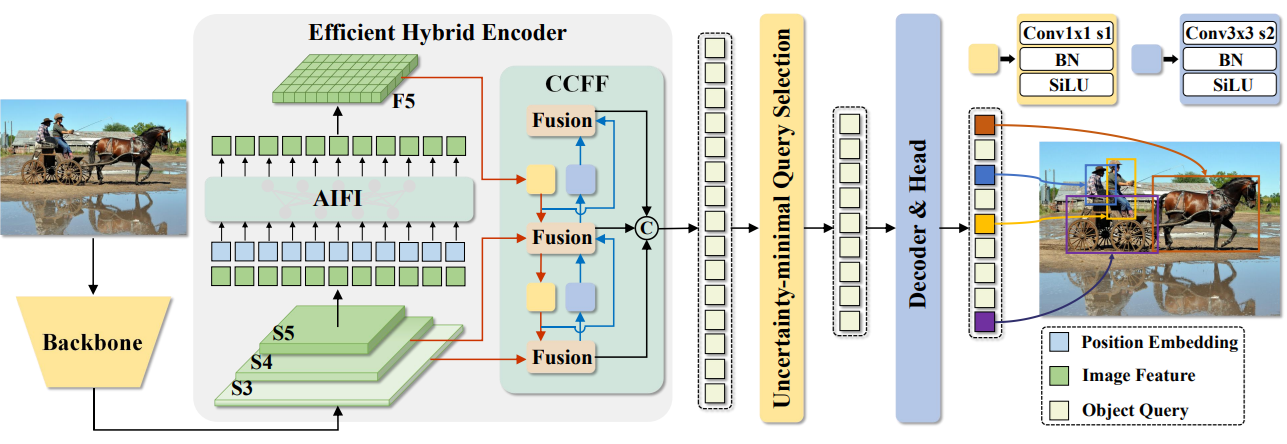
\includegraphics[width=.85\textwidth]{figures/rt-detr.png}
    \caption{Vista general del modelo RT-DETR.\\
    \footnotesize{Fuente: \textit{https://arxiv.org/html/2601.12882v1}}}
    \label{fig:rt-detr}
\end{figure}



\subsection{Tesseract OCR}

Como intérprete y lector del texto de las matrículas, se ha seleccionado Tesseract OCR\cite{tesseractocrTesseractWorlds}. Este motor óptico de reconocimiento de caracteres de código abierto utiliza redes neuronales LSTM \textit{(Long Short Term Memory)} para extraer el texto de las imágenes con un 99\% de precisión en más de 100 idiomas.

Como la librería más popular de los algoritmos OCR (tecnología de inteligencia artificial para buscar y reconocer texto en imágenes), Tesseract trabaja buscando patrones en píxeles, letras, palabras y frases con un enfoque en dos pasos llamado reconocimiento adaptativo resumido en la figura \ref{fig:t-ocr}. Se requiere de una etapa para el reconocimiento de caracteres y una segunda para rellenar las letras de las cuales no estaba seguro el algoritmo, pero que encajan con la palabra, frase o contexto.

\begin{figure}[htb]
\centering
    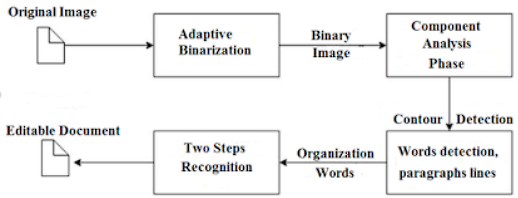
\includegraphics[width=.85\textwidth]{figures/t-ocr.png}
    \caption{Esquema del funcionamiento del algoritmo Tesseract OCR\\
    \footnotesize{Fuente: \textit{https://tesseractocr.blogspot.com/2020/12/how-tesseract-ocr-works.html}}}
    \label{fig:t-ocr}
\end{figure}

El primer paso es un análisis de componentes conectados que guarda los contornos de los componentes y los agrupa en \textit{Blobs} por anidación. Esta etapa, aunque computacionalmente costosa, facilita la detección de texto inverso (como si fuera un contraste de blanco y negro) gracias a la anidación de contornos y las relaciones entre contornos hijo y padre. Los \textit{Blobs} se agrupan a su vez en líneas de texto, y se analizan líneas y regiones para determinar si se trata de texto de espaciado fijo o proporcional. 

Las líneas de texto se descomponen en palabras dependiendo del tipo de espaciado entre caracteres, mientras que el texto con espaciado fijo se descompone en celdas de caracteres; el texto proporcional se descompone en palabras usando espacios fijos y variables. El siguiente paso es el reconocimiento por dos pasos:
\begin{itemize}
    \item En el primer paso se intentan reconocer las palabras; de las que cada una se pasa a un clasificador adaptativo como dato de entrenamiento. Este clasificador ahora tiene más posibilidades de reconocer texto con mayor precisión.
    \item Segundo paso para intentar reconocer las palabras que no se reconocieron con la suficiente claridad. Esta fase resuelve espacios variables y explora alternativas para localizar texto con menor tamaño de fuente.    
\end{itemize}



\chapter{Metodología experimental}
\label{Metodología experimental}

La metodología que se ha empleado es la habitual en el desarrollo de programas relacionados con \textit{Machine Learning} y/o \textit{Deep Learning}, similar al de la figura \ref{fig:metodologia-dl}: (1) Recogida de datos, (2) Procesamiento de los datos, (3) Selección de los modelos, (4) Entrenamiento de los modelos, (5) Validación del modelo y resultados.

\begin{figure}[htb]
\centering
    \includegraphics[width=.85\textwidth]{figures/methodology_dl.jpg}
    \caption{Metodología del diagnóstico y clasificación de Alzheimer con CNNs\\
    \footnotesize{Fuente: \textit{https://peerj.com/articles/cs-1177/}}}
    \label{fig:metodologia-dl}
\end{figure}



\section{Extracción de datos}

Se han investigado y recopilado varios conjuntos de datos desde varias fuente, sobre todo desde Kaggle y Github. Los mejores datasets para el proyecto tendrían que tener tanto imágenes del mismo vehículo desde diferentes ángulos/cámaras como que la matrícula sea legible. Lamentablemente, el tipo de datasets que cumplan ambas funciones son bastante raros, aunque se han podido sacar 2 datasets que lo cumplen y otros dos que, aunque no hay posibilidad de variedad de cámaras hacia el mismo objetivo, aportan con gran cantidad de vehículos y sus matrículas.

\subsection{Multi-perspective traffic video analysis}

Este conjunto de datos \cite{Sanchez-Iborra2026} está comprendido por 3 escenarios distintos, las cuales a su vez se dividen en 3 perspectivas distintas (cámara del coche, dron y cámara de vigilancia), que a su vez cada una se divide en 2 secuencias de vídeo distintas grabadas a una resolución de \textbf{1920 x 1080} a \textbf{60 fotogramas por segundo}; el total de secuencias de vídeo alcanzando 18. Un ejemplo de fotograma del dataset se puede observar en la figura \ref{fig:rsu-esc1}. Ya que este conjunto de datos no trae ningún 

\begin{figure}[htb]
\centering
    \includegraphics[width=.85\textwidth]{figures/rsu_esc1.png}
    \caption{Fotograma del escenario 1 con la perspectiva de una RSU\\
    \footnotesize{Fuente: \textit{https://zenodo.org/records/18375218}}}
    \label{fig:rsu-esc1}
\end{figure}


\subsection{Bdd100k}

Este conjunto de datos \cite{bdd100k} es uno de los más grandes y diversos en cuestión de imágenes de vehículos con anotaciones precisas. Como sugiere el nombre, el dataset consta de 100,000 vídeos grabados desde una cámara acoplada en la parte delantera interior del vehículo; cada uno dura 40 segundos y están grabados a una resolución de \textbf{720 píxeles} a \textbf{30 fps}. Para mantener un dataset diverso, Bdd100k cubre diferentes condiciones climáticas y periodos del día. Las anotaciones incluyen tanto las de detección como las de segmentación y cubren 10 categorías diferentes, como los autobuses y las señales, pudiéndose observar en la figura \ref{fig:bdd} el número de apariciones de cada una de ellas en el dataset. Un ejemplo del conjunto de datos se puede observar en la figura \ref{fig:bdd-example}.

\begin{figure}[htb]
\centering
    \includegraphics[width=.85\textwidth]{figures/bdd100k.png}
    \caption{Estadísticas de los diferentes tipos de objetos en el dataset Bdd100k\\
    \footnotesize{Fuente: \textit{https://bair.berkeley.edu/blog/2018/05/30/bdd/}}}
    \label{fig:bdd}
\end{figure}

\begin{figure}[htb]
\centering
    \includegraphics[width=.85\textwidth]{figures/bdd_example.png}
    \caption{Ejemplo del dataset Bdd100k\\
    \footnotesize{Fuente: \textit{https://www.kaggle.com/datasets/solesensei/solesensei\_bdd100k}}}
    \label{fig:bdd-example}
\end{figure}


\subsection{UC3M-LP}

Este conjunto de datos creado por investigadores de la universidad Carlos III de Madrid \cite{RAMAJOBALLESTER2024104608} es presentado para la tarea de \textbf{detección de matrículas y reconocimiento de caracteres} junto a otro dataset de gran tamaño para reidentificación de vehículos: UC3M-VRI. Se almacenan 1975 imágenes de 2547 vehículos distintos, lo que hacen 2547 matrículas, sumando un total de 12757 caracteres. Algunos ejemplos se pueden observar en la figura \ref{fig:uc3mlp-example}. La variedad de imágenes es amplia en cuestión de luz: 2185 imágenes de día y 362 de noche; la distancia de la cámara al vehículo es de entre 1 y 20 metros y la perspectiva cambia en cada imagen. El conjunto se ha probado en diferentes modelos de detección, incluyendo varias arquitecturas YOLO (varios modelos de los YOLOv3, YOLOv4 y YOLOv5), EfficientDet, ATSS y ASFF, siendo el resultado más notable el de \textbf{YOLO5s} con un tamaño de imagen de \textbf{1280 píxeles}, consiguiendo un \textbf{mAP@0.5 de 98.8\%} y un \textbf{mAP@0.5-0.95 de 89.3\%}. En el caso del reconocimiento de la matrícula, utilizando el mismo modelo con el tamaño de imagen de \textbf{640 píxeles y el optimizador AdamW} se consigue un \textbf{mAP@0.5 de 97.6\%} y un \textbf{mAP@0.5-0.95 de 76.4\%}.

\begin{figure}[htb]
\centering
    \includegraphics[width=.85\textwidth]{figures/uc3mlp_example.png}
    \caption{Ejemplos del dataset UC3M-LP\\
    \footnotesize{Fuente: \textit{https://github.com/ramajoballester/UC3M-LP}}}
    \label{fig:uc3mlp-example}
\end{figure}


\subsection{UC3M-VRI}

Este conjunto de datos es la otra mitad de la investigación del dataset anterior \cite{RAMAJOBALLESTER2024104608} y está orientado a reidentificación de vehículos. Se almacenan 1611 imágenes de 286 vehículos distintos todas sacadas de día y divididas en dos subconjuntos:
\begin{itemize}
    \item \textbf{Conjunto de carretera:} 458 imágenes de 201 vehículos diferentes, sacadas a una distancia de entre 5 a 7 metros con una sola perspectiva.
    \item \textbf{Conjunto de intersección:} 1153 imágenes de 85 vehículos diferentes, sacadas a una distancia de entre 10 y 20 metros usando 2 cámaras para realizar diferentes planos sobre los vehículos que aparecen.
\end{itemize}
Algunos ejemplos se pueden observar en la figura \ref{fig:uc3mlp-example}. Los modelos seleccionados son EfficientNetB0 y FastReid, cada uno con otros 2 modelos que han sido entrenados en datasets diferentes: \textbf{Stanford-Cars} \cite{6755945}, \textbf{VeRi-776} y \textbf{VeRi-Wild}. El modelo con mayores resultados ha sido FastReid (entrenado en VeRi-776) con un 97.9\% de accuracy con el test positivo-negativo (se selecciona una imagen (positiva) y se selecciona una segunda del resto de clases (negativa)) en el subdataset de carreteras y un 87.8\% de accuracy en el subdataset de intersecciones.

\begin{figure}[htb]
\centering
    \includegraphics[width=.85\textwidth]{figures/uc3mvri_example.png}
    \caption{Ejemplos del dataset UC3M-VRI\\
    \footnotesize{Fuente: \textit{https://github.com/ramajoballester/UC3M-VRI}}}
    \label{fig:uc3mvri-example}
\end{figure}



\section{Preprocesado de datos}

Ya que el dataset tenía una estructura diferente a la pedida por los modelos YOLO, se ha creado una función que reconstruya toda esta estructura de forma que quede de la siguiente forma:

\dirtree{%
.1 *.py.
.1 datasets.
.2 bdd100k_yolo.
.3 train1.yaml.
.3 train.
.4 images.
.5 *.jpg.
.4 labels.
.5 *.txt.
.3 test.
.3 val.
.2 UC3M-LP.
}

Ahora que se tienen todas las imágenes para poder entrenar, validar y probar el modelo YOLO, se tienen que transformar las etiquetas por defecto del conjunto de datos al formato \textbf{<class\_id> <center\_x> <center\_y> <width> <height>}, correspondientes al número identificador de la clase, las coordenadas x e y del centro de la \textit{bounding box} y el ancho y altura de esta última. Estos cuatro últimos valores están normalizados al rango [0,1].

Esta estructura es la requerida para YOLO, pero el modelo RT-DETR requiere una estructura COCO (ya que este modelo fue entrenado en este dataset). Sin embargo, esta adición es muy sencilla, pues en vez de tener que generar un archivo \textbf{.txt} por cada imagen, el formato COCO necesita de un archivo \textbf{.json} por cada conjunto (entrenamiento, validación y pruebas) y que se puede transformar directamente con el paquete yolococo y donde el archivo .txt almacena una lista de las clases del dataset en orden y en 3 líneas diferentes. 
\begin{lstlisting}
uv run yolococo yolo2coco --images datasets/bdd100k_yolo/train/images/ --labels datasets/bdd100k_yolo/train/labels --classes classes.txt  --bbox-round 3 --file-name-mode name --out datasets/bdd100k_yolo/train/train.json

uv run yolococo yolo2coco --images datasets/bdd100k_yolo/val/images --labels datasets/bdd100k_yolo/val/labels --classes classes.txt  --bbox-round 3 --file-name-mode name --out datasets/bdd100k_yolo/val/val.json
\end{lstlisting}

El esquema de archivos quedaría de la siguiente manera:
\dirtree{%
.1 *.py.
.1 datasets.
.2 bdd100k_yolo.
.3 train1.yaml.
.3 train.
.4 train.json.
.4 images.
.5 *.jpg.
.4 labels.
.5 *.txt.
.3 test.
.3 val.
.2 UC3M-LP.
}



\section{Entrenamiento}

En este apartado se mostrarán los diferentes parámetros y configuraciones aplicadas o que se han probado en los entrenamientos de los modelos YOLO y DINO-DETR.


\subsubsection{YOLO}

Gracias a Ultralytics \footnote{Toda la información de la librería de Ultralytics es de código abierto y está disponible en \url{https://github.com/ultralytics/ultralytics}}, está a disposición de estudiantes e investigadores una librería entera con montones de recursos para poder entrenar, validar y probar los modelos YOLO. De entre todos los parámetros disponibles, para el entrenamiento de este modelo se han utilizado o experimentado con los siguientes:

\begin{itemize}
    \item \textbf{Model}: Modelo que será entrenado.

    \item \textbf{Data}: Archivo de configuración del dataset con formato \textit{.yaml}. En este archivo se fijan las rutas a las carpetas de entrenamiento, validación y pruebas, el número de clases y la asignación de IDs a cada clase. El archivo usado para entrenar el modelo YOLO se puede observar en la figura \ref{fig:yaml}.

    \item \textbf{Epochs}: Cada época representa una pasada por el dataset entero.
    
    \item \textbf{Time}: Tiempo máximo del entrenamiento. Si este campo no está vacío, se usará en vez del parámetro de las iteraciones.
    
    \item \textbf{Patience}: Número de etapas que hay que esperar antes de parar el entrenamiento durante las cuales las métricas de validación no mejoran.

    \item \textbf{Batch}: El tamaño de lote significa el número de datos de entrenamiento procesadas por el modelo en una sola iteración. En vez de procesarse el dataset entero, este se divide en unos grupos de datos o \textit{batches}.

    \item \textbf{Imgsz}: Tamaño de imagen usado en el entrenamiento. Si las imágenes del conjunto de datos no están a este tamaño se redimensionan antes de introducirlas en el modelo.

    \item \textbf{Device}: Especifica si se quiere usar la \textbf{CPU}, una única \textbf{GPU} o múltiples \textbf{GPUs} para maximizar la eficiencia del modelo y tardar mucho menos en este proceso.

    \item \textbf{Workers}: Número de hilos trabajadores para la carga de datos. Influye especialmente en la velocidad del procesamiento si se está usando la \textit{GPU}.

    \item \textbf{Optimizer}: Escoger el optimizador para el entrenamiento entre \textbf{SGD}, \textbf{Adam}, \textbf{AdamW}, etc. Afecta a la estabilidad y a la velocidad de convergencia. Por defecto, se selecciona por sí solo en función del modelo.
    
    \item \textbf{Multiscale}: Permite redimensionar un paquete de imágenes (por ejemplo, un valor de 0.25 crearía imágenes de 0.75x a 1.25x).

    \item \textbf{Cos\_lr}: Se utiliza un \textit{scheduler} o programador de la tasa de aprendizaje coseno, ajustando la tasa de aprendizaje siguiendo una curva coseno a lo largo de los \textit{epochs} para mejorar la convergencia.

    \item \textbf{Freeze}: Número de primeras capas del modelo a congelar para reducir el número de parámetros entrenables.

    \item \textbf{Lr0}: Tasa de aprendizaje inicial, influye en la rapidez con la que se actualizan los pesos del modelo.

    \item \textbf{Lrf}: Factor de la tasa de aprendizaje, que sirve junto a la tasa de aprendizaje inicial, para calcular la tasa de aprendizaje final de la forma: $lr\_final = lr0 \times lrf$. Se usa en conjunto con el \textit{scheduler} (como el coseno) para ajustar la tasa de aprendizaje a lo largo del entrenamiento.

    \item \textbf{Weight decay}: Valor de regularización L2, que penaliza los pesos grandes para evitar que el modelo se sobreajuste a los datos de entrenamiento (overfitting).

    \item \textbf{Dropout}: Tasa de pérdida de nodos del modelo para la regularización en tareas de clasificación, que evita el sobreajuste omitiendo aleatoriamente unidades durante el entrenamiento.

    \item \textbf{Cache}: Decide si se quiere guardar en memoria RAM o disco las imágenes del conjunto de datos. Mejora la velocidad de entrenamiento a costa de un mayor uso de memoria.

    \item \textbf{Plots}: Dibujar gráficas de las métricas de entrenamiento y validación al acabar de entrenar el modelo. Además, se guardan varias imágenes con las predicciones hechas por el modelo YOLO para comprobar su rendimiento. 

    \item \textbf{Exist\_ok}: Decidir si se sobrescribe la carpeta donde se guardan los archivos de entrenamiento.
    
    \item \textbf{Save}: Decide si se guardan los pesos durante el entrenamiento para fijar puntos de control temporales. Esto permite resumir el entrenamiento a posteriori
    
    \item \textbf{Save\_period}: Cada cuántas épocas se realiza el guardado de pesos.

    \item \textbf{Single\_cls}: El modelo trata todas las clases del archivo de configuración como una sola. Es útil para centrar al modelo en solamente la tarea de detección.
    
    \item \textbf{Project}: Nombre del directorio donde se guardarán los resultados de entrenamiento.
\end{itemize}

\begin{figure}[htb]
\centering
    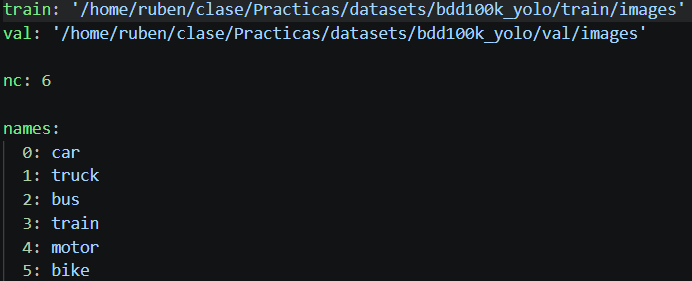
\includegraphics[width=.85\textwidth]{figures/yaml.png}
    \caption{Ejemplo de archivo .yaml de configuración para entrenar un modelo YOLO}
    \label{fig:yaml}
\end{figure}

El entrenamiento de este modelo YOLO consta de:

\begin{lstlisting}
results_val = model.train(data = "./datasets/vehicles/train1.yaml",
                            epochs = 50,
                            device = device,
                            workers = 4, 
                            batch = 16,
                            patience = 25,
                            cos_lr = True,
                            optimizer = "auto",
                            pretrained = False,
                            weight_decay = 0.0001,
                            freeze = 0,
                            verbose = True,
                            plots = True,
                            exist_ok = True,
                            save_period = 25,
                            name = "y26_1",
)
\end{lstlisting}



Es habitual encontrarse este apartado en la sección de preprocesamiento de datos, pero debido a que en este caso del modelo YOLO, se pueden enviar parámetros de data augmentation a través de la misma función que los hiperparámetros:
\begin{itemize}
    \item \textbf{hsv\_h}: Ajusta la tonalidad de la imagen para ayudar al modelo a generalizar ante diferentes condiciones de iluminación. Por defecto, tiene el valor 0.015 (0.0 - 1.0).
    \item \textbf{hsv\_s}: Ajusta la saturación de la imagen para ayudar al modelo a generalizar ante distintos entornos. Por defecto, tiene el valor 0.7 (0.0 - 1.0).
    \item \textbf{hsv\_v}: Ajusta el brillo de la imagen para ayudar al modelo a generalizar ante diferentes condiciones de iluminación. Por defecto, tiene el valor 0.4 (0.0 - 1.0).
    \item \textbf{degrees}: Aplica una rotación aleatoria a la imagen en el rango determinado para ayudar al modelo a reconocer objetos en distintas rotaciones. Por defecto, tiene el valor 0 (0.0 - 180).
    \item \textbf{translate}: Aplica una traslación horizontal y vertical a la imagen por el valor determinado para ayudar al modelo a reconocer objetos parcialmente visibles. Por defecto, tiene el valor 0.1 (0.0 - 1.0).    
    \item \textbf{scale}: Escala la imagen por un valor determinado para ayudar al modelo a reconocer objetos a distintas distancias. Por defecto, tiene el valor 0.5 (0 - 1).
    \item \textbf{shear}: Recorta la imagen por un grado determinado para ayudar al modelo a reconocer objetos desde diferentes ángulos. Por defecto, tiene el valor 0 (-180 - 180).
    \item \textbf{perspective}: Aplica una transformación de perspectiva a la imagen para ayudar al modelo a reconocer objetos en espacios 3D. Por defecto, tiene el valor 0 (0.0 - 0.001).
    \item \textbf{flipud}: Voltea la imagen de arriba hacia abajo con una probabilidad determinada. Por defecto, tiene el valor 0 (0.0 - 1.0).
    \item \textbf{fliplr}: Voltea la imagen de izquierda hacia derecha con una probabilidad determinada para ayudar al modelo a reconocer objetos simétricos. Por defecto, tiene el valor 0 (0.0 - 1.0).
    \item \textbf{bgr}: Cambia los canales de la imagen de RGB a BGR para corregir el desorden de los canales. Por defecto, tiene el valor 0 (0.0 - 1.0).
    \item \textbf{mosaic}: Combina 4 imágenes en una única para ayudar al modelo a entender escenarios complejos. Por defecto, tiene el valor 1 (0.0 - 1.0). 
    \item \textbf{mixup}: Mezcla 2 imágenes y sus etiquetas, creando una imagen compuesta e introduciendo ruido en las etiquetas. Por defecto, tiene el valor 0 (0.0 - 1.0).
    \item \textbf{cutmix}: Combina porciones de 2 imágenes, creando una mezcla parcial con distintas regiones. Por defecto, tiene el valor 0 (0.0 - 1.0). 
    \item \textbf{copy\_paste}: Copia y pega objetos entre imágenes. Por defecto, tiene el valor 0 (0.0 - 1.0). 
    \item \textbf{copy\_paste\_mode}: Especifica el modo de copia y pega. Por defecto, tiene el valor \textit{flip} (flip/mixup).
    \item \textbf{auto\_augment}: Aplica un aumento a la imagen. Por defecto, tiene el valor \textit{randaugment} (randaugment/autoaugment/augmix).
    \item \textbf{erasing}: Borra regiones aleatorias de la imagen para ayudar al modelo a enfocarse en características menos obvias. Por defecto, tiene el valor 0.4 (0.0 - 1.0).
\end{itemize}



\subsubsection{DINO-DETR}

Gracias a la librería de \textbf{Huggingface}, \textbf{transformers}\footnote{Toda la información de la librería de transformers es de código abierto y está disponible en \url{https://huggingface.co/docs/transformers}}, está a disposición de estudiantes e investigadores una librería entera con montones de recursos para poder entrenar y validar diferentes tipos de transformadores. De entre todos los parámetros disponibles, para el entrenamiento de este modelo se han utilizado o experimentado con los siguientes:
\begin{itemize}
    \item \textbf{output\_dir}: 
    \item \textbf{per\_device\_train\_batch\_size} y \textbf{per\_device\_val\_batch\_size}: Tamaño de lote por dispositivo. 
    \item \textbf{num\_train\_epochs}: Número total de iteraciones sobre los conjuntos de entrenamiento y validación.
    \item \textbf{learning\_rate}: Tasa de aprendizaje inicial del optimizador.
    \item \textbf{lr\_scheduler\_type}: Tipo de optimizador de la tasa de aprendizaje que se va a usar.
    \item \textbf{warmup\_steps}: Número de iteraciones para que la tasa de aprendizaje pase de 0 al valor fijado por el anterior parámetro.
    \item \textbf{optim}: Optimizador que se va a usar.
    \item \textbf{weight\_decay}: Valor de regularización L2, que penaliza los pesos grandes para evitar que el modelo se sobreajuste a los datos de entrenamiento (overfitting).
    \item \textbf{gradient\_accumulation\_steps}: Pasos de actualización para acumular gradientes antes de hacer el pase \textit{backward/update}. Simula grandes lotes sin memoria adicional.
    \item \textbf{fp16}: Activa el entrenamiento de precisión mixto float16 (FP16).
    \item \textbf{logging\_strategy}: Estrategía de generación de \textit{logs} 
\end{itemize}

Los parámetros de entrenamiento utilizados se enumeran a continuación:

\begin{lstlisting}
training_args = TrainingArguments(
    output_dir="/kaggle/working/rtdetr-custom",
    per_device_train_batch_size=20,
    per_device_eval_batch_size=20,
    gradient_accumulation_steps=2,
    dataloader_num_workers=4,
    num_train_epochs=30,
    learning_rate=1e-5,
    logging_steps=50,
    save_steps=500,
    eval_strategy="epoch",
    save_strategy="epoch",
    remove_unused_columns=False,
    fp16=True,
    load_best_model_at_end=True,
    metric_for_best_model="eval_loss",
    greater_is_better=False,
    save_total_limit=3,
    lr_scheduler_type="cosine",
    warmup_steps=50,
    weight_decay=0.05,
)
\end{lstlisting}



\subsection{Rastreo del Overfitting}

Con el objetivo de evaluar el rendimiento del modelo y detectar posibles indicios de sobreajuste durante el entrenamiento, se ha realizado un seguimiento detallado de los valores de pérdida (loss\_rates), los cuales se registraron durante el entrenamiento en cada iteración en los conjuntos de entrenamiento y validación. El análisis de estas gráficas permite observar el comportamiento del modelo y determinar si está memorizando los datos de entrenamiento en lugar de generalizar correctamente.

En los experimentos realizados se ha prestado especial atención a la diferencia entre las pérdidas tanto de entrenamiento como de validación ya que dependiendo del diferencial entre ellas podría llevar al sobreajuste. Estas pérdidas se extraen de un archivo csv creado automáticamente por el entrenamiento del modelo YOLO, que, a cada iteración extrae las siguientes métricas: \textbf{epoch, time, train/box\_loss, train/cls\_loss, train/dfl\_loss, metrics/precision(B), metrics/recall(B), metrics/mAP50(B), metrics/mAP50-95(B), val/box\_loss, val/cls\_loss y val/dfl\_loss}. Aunque es muy útil seguir la evolución de las métricas como precision, recall o mAP50-95, para rastrear signos de overfitting o underfitting. En la figuras \ref{fig:g-ms} y \ref{fig:g-no-ms} se pueden ver dos configuraciones diferentes de entrenamiento para la detección de vehículos: en la primera figura se utiliza el parámetro \textit{multiscale}, que redimensiona las imágenes por cierto valor durante el entrenamiento, mientras que en la segunda no se utiliza este parámetro. De valores similares, ambas gráficas dotan de un problema: el underfitting; en ambas gráficas la pérdida de validación se mantiene inferior a la de entrenamiento, lo que significa que el modelo tenía demasiada penalización durante el entrenamiento. 

\begin{figure}[htb]
\centering
    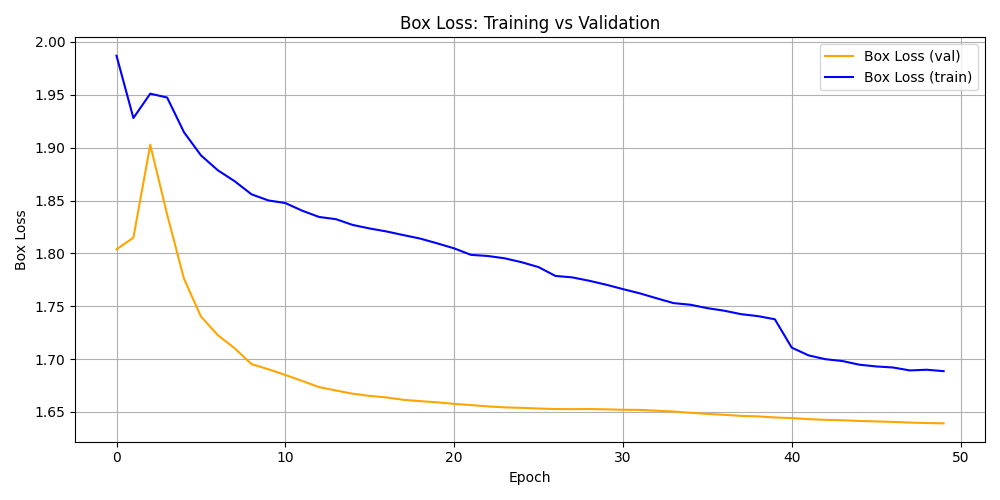
\includegraphics[width=.85\textwidth]{figures/g_no_ms.png}
    \caption{Gráfica de la evolución de las pérdida de detección de entrenamiento y validación sin multiscale}
    \label{fig:g-no-ms}
\end{figure}

\begin{figure}[htb]
\centering
    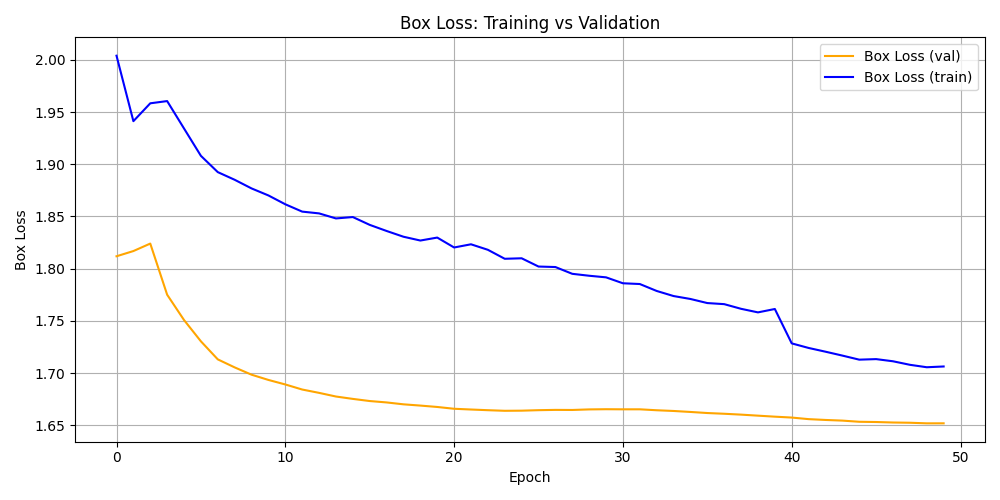
\includegraphics[width=.85\textwidth]{figures/g_ms.png}
    \caption{Gráfica de la evolución de las pérdida de detección de entrenamiento y validación con multiscale}
    \label{fig:g-ms}
\end{figure}

\section{Métricas}

Para poder validar de forma equitativa los distintos métodos de detección, se tienen que seguir unas métricas a seguir para todos. Para empezar, se tiene que hablar del tiempo de procesamiento por imagen, ya que la velocidad de inferencia es prioritaria a la hora de detectar y reconocer claramente el vehículo y su matrícula.

\begin{itemize}
    \item \textbf{mAP50}: Precisión media de las detecciones, calculada con un umbral de intersección (IoU) de 0,5.

    \item \textbf{mAP50-95}: Media entre todas las precisiones medias entre el umbral IoU 0,50 y 0,95, ambos umbrales incluidos.

    \item \textbf{Precisión}: En una clase, es el número de predicciones correctas para esta clase entre el número total de predicciones para esta misma clase.

    \item \textbf{Recall}: En una clase, es el número de predicciones correctas para esta clase entre el número total de instancias de esta misma clase.

    \item \textbf{F1-score}: Es una métrica especializada para cuando las clases están desbalanceadas, es decir, el número de instancias de cada clase no es el mismo para cada una. Se calcula primero para cada clase con la ecuación:
    \begin{gather*}
        F1score = 2 \times \dfrac{Precision \times Recall}{Precision + Recall}
    \end{gather*}
\end{itemize}

En el caso de las métricas de Precision, Recall y F1-score, para hacer la media del dataset entero hay dos opciones: (1) \textbf{Macro}: El sumatorio del \textit{f1-score} de cada clase entre el número de clases y (2) \textbf{Ponderada}: Considerar el número de instancias de cada clase, siendo las clases con mayor número de imágenes las que más aportan a la media.

Además de estas métricas, se analizará también la diferenciación entre clases, es decir, fallos al clasificar correctamente la categoría de cada vehículo detectado. Esto se podría visualizar a través de la pérdida de clasificación en el entrenamiento, por ejemplo, pero se va a usar una matriz de confusión como la de la figura \ref{fig:cm} para ver que problemas tienen los modelos en situaciones donde no solo el modelo tenga problemas para detectar el vehículo, sino también para identificar exactamente qué es.

\begin{figure}[htb]
\centering
    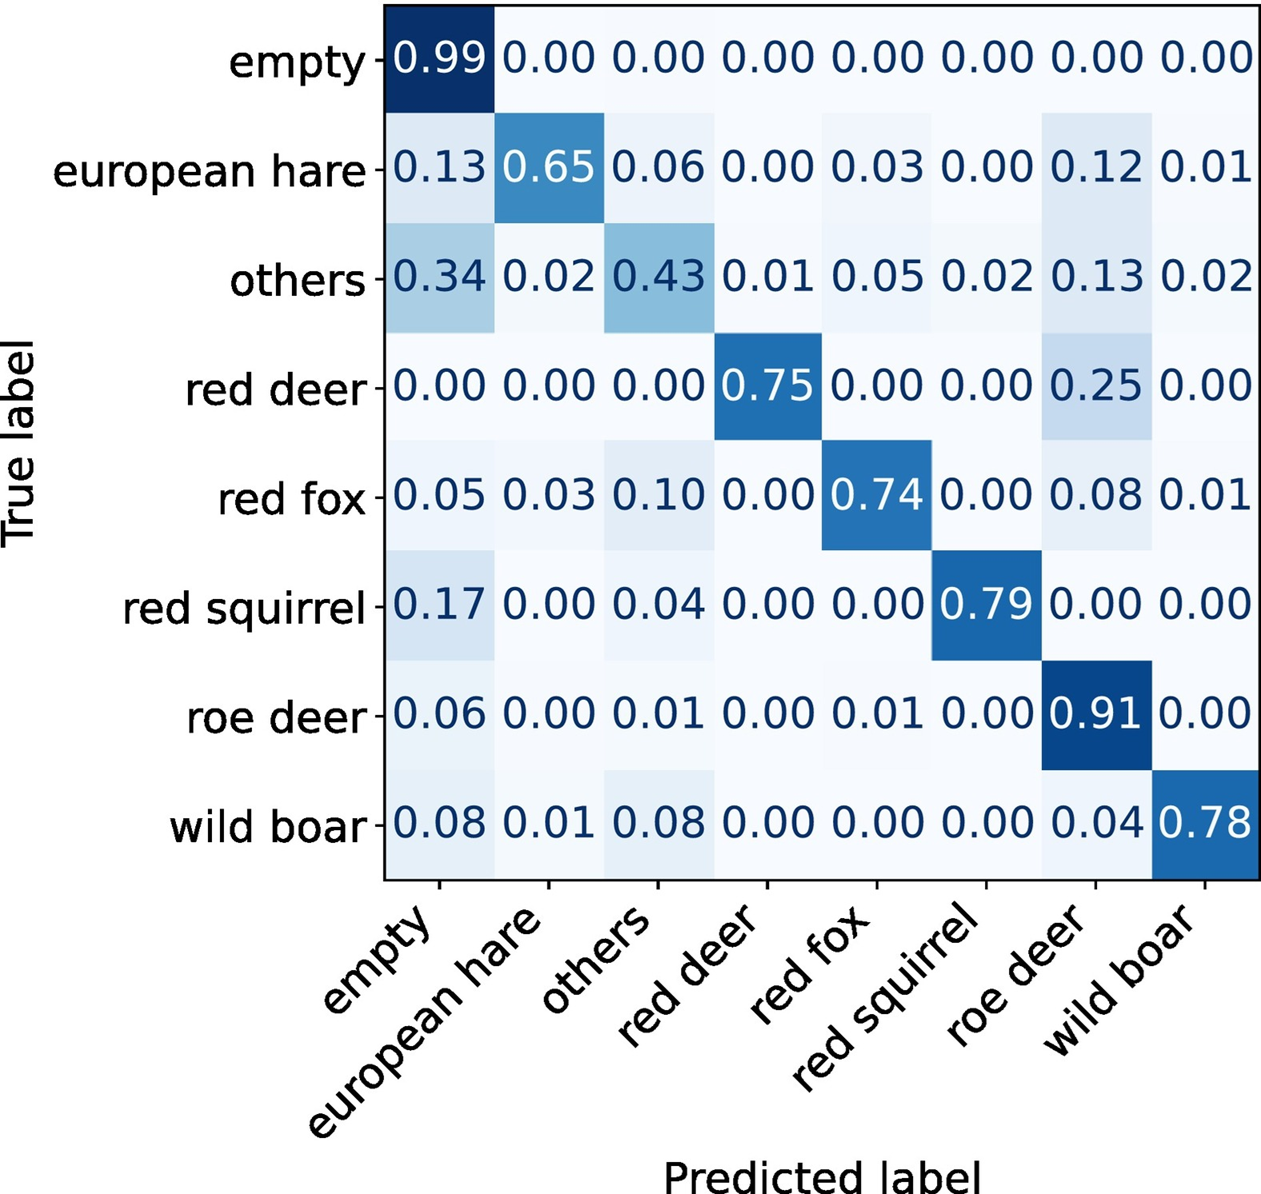
\includegraphics[width=0.85\textwidth]{figures/confmatrix.png}
    \caption{Ejemplo de matriz de confusión}
    \label{fig:cm}
\end{figure}




\chapter{Resultados experimentales}
\label{Resultados experimentales}

En este apartado se presentan los resultados obtenidos tras el entrenamiento, evaluación y pruebas de los distintos modelos de detección de vehículos y matrículas. Se comparan los rendimientos alcanzados por cada método, así como la precisión en la inferencia sobre las imágenes de prueba. Para ello, como antes se explicó en la extracción de datos, se utiliza el subconjunto de pruebas del dataset CCPD para calcular estos resultados.


\section{Resultados de rendimiento}

El apartado de rendimiento de un modelo es muy importante debido a la necesidad de generar predicciones de detección de objetos de forma lo más rápida posible, casi instantáneamente. En la tabla \ref{Res-Rendimiento} se comparan los modelos utilizados en función de estas métricas: (1) \textbf{Tiempo medio por imagen}, (2) \textbf{Tiempo en total} del dataset, y (3) \textbf{Frames Por Segundo (FPS)} que son capaces de ejecutar de forma constante.

\begin{table}[ht]
    \centering
    \caption{Resultados de rendimiento}
    \begin{tabular}{|c|c|c|c|}
        \hline
        \textbf{Método} & \textbf{Tiempo por imagen} & \textbf{Tiempo total} & \textbf{FPS}\\
        \hline
        \textbf{YOLOv26} & 0 ms & 0 s & 0 FPS\\
        \hline
        \textbf{RT-DETR} & 0 ms & 0 s & 0 FPS\\
        \hline
    \end{tabular}
    \label{Res-Rendimiento}
\end{table}


\section{Resultados de detección de vehículos}

En este apartado, el principal objetivo es detectar correctamente los vehículos que salgan en la imagen. La tabla \ref{Res-Deteccion-V} detalla los resultados obtenidos.

\begin{table}[ht]
    \centering
    \caption{Resultados de detección}
    \begin{tabular}{|c|c|c|c|c|c|}
        \hline
        \textbf{Método} & \textbf{Precision} & \textbf{Recall} & \textbf{F1-score} & \textbf{mAP50} & \textbf{mAP50-95}\\
        \hline
        \textbf{YOLOv26n} & 0\% & 0\% & 0\% & 0\% & 46.12\%\\
        \hline
        \textbf{RT-DETR} & 0\% & 0\% & 0\% & 0\% & 0\%\\
        \hline
    \end{tabular}
    \label{Res-Deteccion-V}
\end{table}


\section{Resultados de detección de matrículas}

En este apartado, el principal objetivo es detectar correctamente el entorno de la matrícula de los vehículos que salgan en la imagen. La tabla \ref{Res-Deteccion-LP} detalla los resultados obtenidos.

\begin{table}[ht]
    \centering
    \caption{Resultados de detección}
    \begin{tabular}{|c|c|c|c|c|c|}
        \hline
        \textbf{Método} & \textbf{Precision} & \textbf{Recall} & \textbf{F1-score} & \textbf{mAP50} & \textbf{mAP50-95}\\
        \hline
        \textbf{YOLOv26n} & 0\% & 0\% & 0\% & 0\% & 46.12\%\\
        \hline
        \textbf{RT-DETR} & 0\% & 0\% & 0\% & 0\% & 0\%\\
        \hline
    \end{tabular}
    \label{Res-Deteccion-LP}
\end{table}


\section{Limitaciones detectadas}

Aunque los resultados globales son satisfactorios, ... %TODO


\section{Modelo seleccionado}

El método seleccionado ha sido la integración del modelo \textbf{X} para vehículos y el modelo \textbf{Y} . Ambos se integran en una aplicación web que permite la carga de imágenes o la lectura desde cámara en tiempo real. Tras comparar varias configuraciones de modelos, se optó por usar esta combinación por ofrecer los mejores resultados de detección y rendimiento. %TODO
 
... %TODO

Esta configuración, ... , es la más óptima para este proyecto y su integración en la aplicación web.



\chapter{Aplicación web}
\label{Aplicación web}

...


\section{El producto de desarrollo}

Casos de uso...



\chapter{Legislación y normativa}
\label{Legislación y normativa}

\section{Normativa nacional}

\begin{itemize}
    \item \textbf{Ley de acceso electrónico de los ciudadanos a los Servicios Públicos} \url{https://boe.es/buscar/pdf/2007/BOE-A-2007-12352-consolidado.pdf}. Reconocimiento de los ciudadanos a relacionarse con las entidades públicas por vía electrónica, asegurando la disponibilidad, el acceso, la integridad, la confidencialidad y la conservación de los datos y servicios que gestionen: No aplica debido a que esta aplicación no pertenece ni hay una relación con las Administraciones Públicas.
    
    \item \textbf{Real Decreto sobre accesibilidad de los sitios web y aplicaciones para dispositivos móviles del sector público} \url{https://www.boe.es/buscar/pdf/2018/BOE-A-2018-12699-consolidado.pdf}. Derecho a la accesibilidad de la información textual y no textual, documentos y formularios, contenidos multimedia y los procesos de identificación, autenticación, firma y pago para garantizar la igualdad de todas los usuarios (sin discriminar a ninguno): No se puede aplicar esta normativa a este proyecto debido a que está sujeto al sector público. Sin embargo, se han intentado seguir las recomendaciones de accesibilidad en la medida de lo posible para este tipo de proyectos.
    
    \item \textbf{Esquema nacional de interoperabilidad} \url{https://www.boe.es/buscar/pdf/2010/BOE-A-2010-1331-consolidado.pdf}. Asegurar los criterios y recomendaciones de seguridad, normalización y conservación de la información en la administración pública: Esta ley no es aplicable tampoco para esta aplicación, al tener el mismo ámbito de aplicación que la Ley 11/2007, de 22 de junio y explicado en el primer punto. 
    
    \item \textbf{Esquema nacional de seguridad} \url{https://www.boe.es/diario_boe/txt.php?id=BOE-A-2022-7191}. Proteger la información tratada y los servicios prestados por las entidades con objeto de asegurar el acceso, la confidencialidad, la integridad, la autenticidad, la disponibilidad y la conservación de los datos: Este esquema no se puede aplicar por los siguientes motivos: (1) No se pertenece ni hay relación con el sector público y (2) No se trata información clasificada.
    
    \item \textbf{Ley Orgánica de protección de datos personales y garantía de los derechos digitales} \url{https://www.boe.es/boe/dias/2018/12/06/pdfs/BOE-A-2018-16673.pdf}. Respetar el tratamiento de los datos personales de las personas físicas y la libre circulación de estos: La ley orgánica de datos personales no se puede aplicar debido a que no se recolectan ni se usan datos personales de ningún tipo.
    
    \item \textbf{Reglamento General de Protección de Datos} \url{https://www.boe.es/doue/2016/119/L00001-00088.pdf}. Establecer las normativas para la protección y libre circulación de los datos personales de las personas físicas: Al igual que en la ley del punto anterior, no se utilizan datos personales de ningún tipo.

    \item \textbf{Ley de Propiedad Intelectual} \url{https://www.boe.es/boe/dias/2019/03/02/pdfs/BOE-A-2019-2974.pdf}: Durante el desarrollo de este proyecto se han utilizado imágenes, datasets y modelos de redes neuronales que pueden estar protegidos por la legislación vigente. Se ha procurado en todo momento citar adecuadamente las fuentes utilizadas y no vulnerar los derechos de autor. Asimismo, cualquier contenido generado a partir de estos recursos ha sido producido de forma original dentro del marco del proyecto.
\end{itemize}


\section{Licencias}

Los modelos y datasets utilizados durante el desarrollo de este proyecto tienen una serie de licencias a atribuir, incluso teniendo en cuenta el objetivo académico y experimental de este proyecto.

Para empezar, la citación de los cinco datasets utilizados, los cuales

Se ha utilizado un modelo \textbf{YOLO} diferentes desarrollados por Ultralytics. Ambos han sido proporcionados a través de su framework con el mismo nombre.

\begin{itemize}
    \item \textbf{Fuente}: \url{https://github.com/ultralytics/ultralytics}

    \item \textbf{AGPL 3.0 Software License o Ultralytics License}

    \item \textbf{Permisos}: Uso libre para fines académicos o no comerciales. Para uso comercial, sería necesario solicitar una licencia específica a Ultralytics. La redistribución o modificación requiere atribución y mantener el mismo tipo de licencia.
\end{itemize}

Todos los modelos utilizados han sido integrados respetando sus respectivas licencias. En ningún momento se ha modificado su arquitectura interna ni se han distribuido fuera del entorno local de desarrollo. Su uso se limita a un entorno académico y experimental, en el contexto de un Trabajo de Fin de Máster.



\chapter{Gestión de proyecto software}
\label{Gestión de proyecto software}

\section{Diseño del sistema}

La arquitectura general del sistema sigue...


\section{Control de versiones}

Se ha utilizado el sistema de control de versiones \textbf{Git}, en combinación con la plataforma \textbf{GitHub} para almacenar y organizar todo el desarrollo del proyecto. Todo el código para entrenar, validar y probar los diferentes modelos se encuentra en el repositorio de este proyecto: \url{https://github.com/RubenFdezGlez/TFM}. Debido al objetivo experimental de este trabajo, solamente se han utilizado confirmaciones secuenciales en la rama principal \textit{main}. En este repositorio se almacenan únicamente los ejecutables y otros archivos necesarios (como los requisitos de instalación), por lo que los archivos grandes como los datasets no se encuentran aquí.

A lo largo del desarrollo se han realizado varios \textit{commits}, con el fin de registrar los cambios en el desarrollo del proyecto mediante confirmaciones descriptivas como la de la figura \ref{fig:git} que permiten volver atrás o revisar el historial.

\begin{figure}[htb]
\centering
    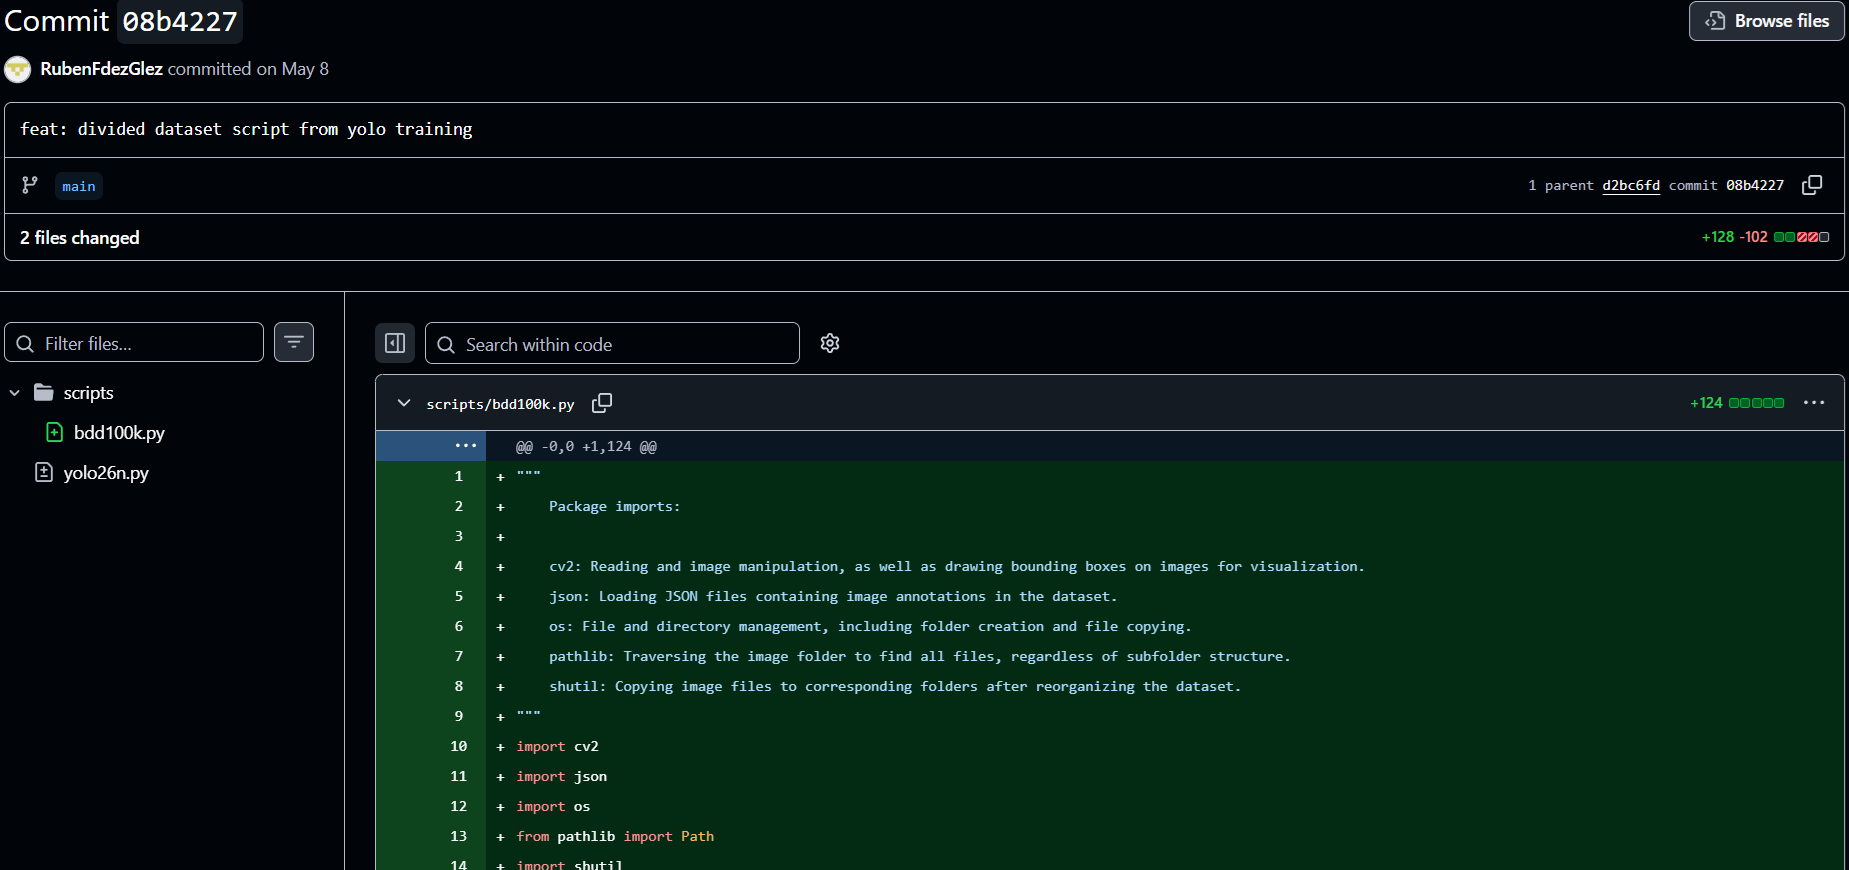
\includegraphics[width=.85\textwidth]{figures/git.png}
    \caption{Ejemplo de commit en GitHub}
    \label{fig:git}
\end{figure}



\section{Requisitos del sistema}

Esta sección sirve para definir qué debe hacer el sistema y cómo debe comportarse o en qué condiciones debe funcionar. 

\subsection{Requisitos funcionales}

Las acciones concretas que el sistema debe ser capaz de realizar se describen en la tabla...



\subsection{Requisitos no funcionales}

Las condiciones de calidad bajo las que debe funcionar el sistema se describen en la tabla...



\section{Planificación del trabajo}
\label{Plan de trabajo}

En esta sección se describe la planificación temporal y técnica del proyecto, con el fin de estructurar de forma ordenada las fases de desarrollo, facilitar el seguimiento de los avances y optimizar los recursos disponibles. Para ello, se ha seguido un enfoque basado en fases iterativas de desarrollo y prueba.

Para el desarrollo del proyecto se han seguido las siguientes fases:

\begin{enumerate}
    \item \textbf{Estudio inicial}: ...

    \item \textbf{Preparación y preprocesamiento del dataset}: ...

    \item \textbf{Entrenamiento de modelos}: ...

    \item \textbf{Evaluación}: ...

    \item \textbf{Implementación web}: ...

    \item \textbf{Documentación}: ...
\end{enumerate}

\section{Cronograma}

El desarrollo ha durado en torno a los cinco meses. La tabla \ref{Actividades} indica las duraciones de cada una de las fases y en la figura ... se muestra el cronograma del proyecto a lo largo de los meses.

\begin{table}[ht]
    \centering
    \caption{Duración de las partes del proyecto (en días)}
    \begin{tabular}{|c|c|c|c|}
        \hline
        \textbf{Tarea} & \textbf{Duración} & \textbf{Fecha de inicio} & \textbf{Fecha final}\\
        \hline
        Estado del arte & . & . & .\\
        \hline
        Preparación del dataset & . & . & .\\
        \hline
        Entrenamiento de modelos & . & . & .\\
        \hline
        Evaluación & . & . & .\\
        \hline
        Implementación web & . & . & .\\
        \hline
        Documentación & . & . & .\\
        \hline
    \end{tabular}
    \label{Actividades}
\end{table}



\section{Presupuesto}

En una empresa o desarrollo dirigido a hacer un producto o servicio, tener en cuenta los costes de desarrollo y mantenimiento de un proyecto es primordial para cualquier empresa que desarrolle software. En la tabla ... se puede visualizar el coste total del trabajo.

\subsection{Coste hardware}

Para el desarrollo del proyecto se utilizaron dos equipos diferentes explicados en el apartado \ref{Entorno y herramientas}. El coste de estos equipos se puede observar en la tabla ....


Ya que los equipos tienen mayor vida útil que la duración de este trabajo, al coste total se le resta una porción de este coste \textbf{(costo imputable)} en función de su uso. El \textbf{costo final (Cf)} es una cantidad equivalente a la guiada por esta fórmula:

\begin{gather*}
    Cf = (C \times U \times D) / P 
\end{gather*}

Donde:
\begin{itemize}
    \item \textbf{Coste (C)}: Coste total (PVP) del producto.
    
    \item \textbf{\% Uso (U)}: Porcentaje de uso que se le da al producto durante el desarrollo.
    
    \item \textbf{Dedicación (D)}: Cantidad de tiempo que se usa el producto.
    
    \item \textbf{Periodo de deprecación (P)}: Periodo de garantía del producto según el fabricante.
\end{itemize}

El costo real para este proyecto, suponiendo que los equipos van a estar en uso un 100\% del tiempo durante un periodo de dedicación de 4 meses, se ve reflejado en la tabla ... .


\subsection{Coste de personal}

En la siguiente tabla ... se refleja el sueldo bruto \footnote{Los sueldos brutos se han obtenido de la página web \url{https://www.salaryexpert.com/salary/job/artificial-intelligence-engineer/spain}} que perciben los empleados durante el desarrollo del proyecto; junto a los costes de la seguridad social y los costes del empleador (se fijan 4 meses).

Los costes de la seguridad social y del empleador se han sacado de la página de Cuestiones Laborales \footnote{\url{https://www.cuestioneslaborales.es/porcentaje-de-cotizacion-a-la-seguridad-social-del-trabajador-y-empresa/}}. Donde la cotización a cargo de la empresa se divide en: \textbf{(2)} Cotizaciones comunes (23,6\%) y \textbf{(1)} Formación, desempleo, FOGASA, accidentes, etc. (en torno al 6,3\%).



\subsection{Coste software}

En la tabla ... se enumeran los recursos software utilizados durante el desarrollo del proyecto. Ya que todos estos fueron gratuitos o de código abierto, no tuvieron repercusión alguna en el coste. Si se desplegara este mismo proyecto en un entorno privado, habría que añadirle como mínimo la licencia de Ultralytics, con un costo aproximado de 150€. Otros posibles costos adicionales podrían ser un sistema de almacenamiento en la nube o un servidor donde desplegar el programa web.



\section{Gestión de riesgos}

A lo largo del desarrollo de este proyecto, se han identificado distintos factores que podrían comprometer su ejecución, resultados y tiempos de entrega.  La tabla \ref{Gestion-riesgos} recoge los principales riesgos detectados, junto con su impacto y probabilidad. En las siguientes tablas (\ref{R1}, \ref{R2}, \ref{R3}, \ref{R4}, \ref{R5}, \ref{R6}, \ref{R7}, \ref{R8}) se muestra: para cada riesgo, sus causas y estrategias a seguir para mitigarlo.

\begin{table}[ht]
    \centering
    \caption{Gestión de riesgos por categoría}
    \begin{tabular}{|c|c|c|c|c|}
        \hline
        \textbf{ID} & \textbf{Riesgo} & \textbf{Categoría} & \textbf{Impacto} & \textbf{Probabilidad}\\
        \hline
        R1 & Incompatibilidad entre librerías & Técnico & Alta & Baja\\
        \hline
        R2 & Errores de memoria & Rendimiento & Alta & Alta\\
        \hline
        R3 & Dataset con errores & Formato & Alta & Media\\
        \hline
        R4 & Pérdida de datos & Humano & Alta & Muy Baja\\
        \hline
        R5 & Errores al integrar modelos & Técnico & Media & Media\\
        \hline
        R6 & Tiempo insuficiente & Humano & Alta & Media\\
        \hline
        R7 & Escasa precisión & Técnico & Alta & Alta\\
        \hline
        R8 & Overfitting en el entrenamiento & Técnico & Alta & Media\\
        \hline
    \end{tabular}
    \label{Gestion-riesgos}
\end{table}

\begin{table}[ht]
    \centering
    \caption{Riesgo incompatibilidad entre librerías}
    \begin{tabularx}{1\textwidth}{| >{\centering\arraybackslash}X | >{\centering\arraybackslash}X |}
        \hline
        \multicolumn{2}{|c|}{\textbf{R1}}\\
        \hline 
        \textbf{Causa} &  Diferencias entre versiones entre PyTorch, Ultralytics, etc.\\
        \hline 
        \textbf{Estrategia de mitigación} & Revisión manual de las versiones de las librerías de modelos que pudieran generar conflictos.\\
        \hline
    \end{tabularx}
    \label{R1}
\end{table}

\begin{table}[ht]
    \centering
    \caption{Riesgo errores de memoria}
    \begin{tabularx}{1\textwidth}{| >{\centering\arraybackslash}X | >{\centering\arraybackslash}X |}
        \hline
        \multicolumn{2}{|c|}{\textbf{R2}}\\
        \hline 
        \textbf{Causa} & Sobrecarga de GPU o errores CUDA. Uso intensivo de la gráfica durante el entrenamiento. Limpieza de memoria de GPU o CPU no realizada efectivamente.\\
        \hline 
        \textbf{Estrategia de mitigación} & Implementación de limpieza automática de la RAM a través de la librería \textit{PyTorch}.\\
        \hline
    \end{tabularx}
    \label{R2}
\end{table}

\begin{table}[ht]
    \centering
    \caption{Riesgo dataset con errores}
    \begin{tabularx}{1\textwidth}{| >{\centering\arraybackslash}X | >{\centering\arraybackslash}X |}
        \hline
        \multicolumn{2}{|c|}{\textbf{R3}}\\
        \hline 
        \textbf{Causa} &  Dataset con etiquetas, imágenes o errores en su estructura.\\
        \hline 
        \textbf{Estrategia de mitigación} & Script para la revisión automática para revisar el dataset entero en busca de errores en las etiquetas, carpetas y otro tipo de fallos en el conjunto de datos.\\
        \hline
    \end{tabularx}
    \label{R3}
\end{table}

\begin{table}[ht]
    \centering
    \caption{Riesgo pérdida de datos}
    \begin{tabularx}{1\textwidth}{| >{\centering\arraybackslash}X | >{\centering\arraybackslash}X |}
        \hline
        \multicolumn{2}{|c|}{\textbf{R4}}\\
        \hline 
        \textbf{Causa} &  Fallos de disco al guardar o errores humanos.\\
        \hline 
        \textbf{Estrategia de mitigación} & Guardado periódico en el repositorio con cambios importantes. Impresión de registros con las ejecuciones.\\
        \hline
    \end{tabularx}
    \label{R4}
\end{table}

\begin{table}[ht]
    \centering
    \caption{Riesgo errores al integrar modelos}
    \begin{tabularx}{1\textwidth}{| >{\centering\arraybackslash}X | >{\centering\arraybackslash}X |}
        \hline
        \multicolumn{2}{|c|}{\textbf{R5}}\\
        \hline 
        \textbf{Causa} &  Modelos incompatibles entre sí o en Flask.\\
        \hline 
        \textbf{Estrategia de mitigación} & Comprobación de las librerías necesarias y pruebas de compatibilidad.\\
        \hline
    \end{tabularx}
    \label{R5}
\end{table}

\begin{table}[ht]
    \centering
    \caption{Riesgo tiempo insuficiente}
    \begin{tabularx}{1\textwidth}{| >{\centering\arraybackslash}X | >{\centering\arraybackslash}X |}
        \hline
        \multicolumn{2}{|c|}{\textbf{R6}}\\
        \hline 
        \textbf{Causa} &  Retrasos en fases anteriores.\\
        \hline 
        \textbf{Estrategia de mitigación} & Optimización de las pruebas y del tiempo requerido.\\
        \hline
    \end{tabularx}
    \label{R6}
\end{table}

\begin{table}[ht]
    \centering
    \caption{Riesgo escasa precisión}
    \begin{tabularx}{1\textwidth}{| >{\centering\arraybackslash}X | >{\centering\arraybackslash}X |}
        \hline
        \multicolumn{2}{|c|}{\textbf{R7}}\\
        \hline 
        \textbf{Causa} &  Sobreajuste, datos insuficientes o mal preprocesamiento.\\
        \hline 
        \textbf{Estrategia de mitigación} & Optimización al cambiar hiperparámetros durante el entrenamiento. Validación cruzada para parar antes el entrenamiento.\\
        \hline
    \end{tabularx}
    \label{R7}
\end{table}

\begin{table}[ht]
    \centering
    \caption{Riesgo overfitting en el entrenamiento}
    \begin{tabularx}{1\textwidth}{| >{\centering\arraybackslash}X | >{\centering\arraybackslash}X |}
        \hline
        \multicolumn{2}{|c|}{\textbf{R8}}\\
        \hline 
        \textbf{Causa} &  Dataset de pequeño tamaño o imágenes demasiado similares.\\
        \hline 
        \textbf{Estrategia de mitigación} & Ampliación de datos con cambios de color, tamaño, contraste, etc.\\
        \hline
    \end{tabularx}
    \label{R8}
\end{table}

La identificación y gestión de estos riesgos ha permitido anticipar problemas y tomar las decisiones proactivas necesarias, asegurando la continuidad del desarrollo y minimizando su impacto en los objetivos del proyecto.





\chapter{Conclusión y posibles mejoras}
\label{Conclusión}

El proyecto ha cumplido con los objetivos planteados, demostrando la viabilidad técnica de aplicar redes neuronales al problema de la detección, identificación y análisis de vehículos. Los resultados obtenidos avalan la validez del enfoque y asientan una base sólida para futuras ampliaciones. Posibles mejoras permitirían incrementar la precisión y escalabilidad del sistema en distintos escenarios.



\section{Problemas encontrados}

A pesar de los buenos resultados...



\section{Mejoras y ampliación a futuro}

Algunas de las propuestas de mejora aplicables a este proyecto pueden ser:

\begin{itemize}
    \item ...
\end{itemize}



\section{Agradecimientos}

Quiero expresar mi más sincero agradecimiento a mi tutor...

También agradecer a ...



%%%% BIBLIOGRAFÍA %%%%
\renewcommand\bibname{Lista de referencias}
\bibliographystyle{splncs04} % Fichero con el formato de la bibliografía.
\bibliography{references}

\end{document}